%%%%%%%%%%%%%%%%%%%%%%%%%%%%%%%%%%%%%%%%%
% Masters/Doctoral Thesis 
% LaTeX Template
% Version 1.43 (17/5/14)
%
% This template has been downloaded from:
% http://www.LaTeXTemplates.com
%
% Original authors:
% Steven Gunn 
% http://users.ecs.soton.ac.uk/srg/softwaretools/document/templates/
% and
% Sunil Patel
% http://www.sunilpatel.co.uk/thesis-template/
%
% License:
% CC BY-NC-SA 3.0 (http://creativecommons.org/licenses/by-nc-sa/3.0/)
%
% Note:
% Make sure to edit document variables in the Thesis.cls file
%
%%%%%%%%%%%%%%%%%%%%%%%%%%%%%%%%%%%%%%%%%

%----------------------------------------------------------------------------------------
%	PACKAGES AND OTHER DOCUMENT CONFIGURATIONS
%----------------------------------------------------------------------------------------

\documentclass[11pt, oneside]{Thesis} % The default font size and one-sided printing (no margin offsets)

\graphicspath{{Pictures/}} % Specifies the directory where pictures are stored

\usepackage{adjustbox}
\usepackage{pdflscape}
\usepackage{afterpage}
\usepackage{tikz}
\usetikzlibrary{positioning}
\usepackage[square, numbers, comma, sort&compress]{natbib} % Use the natbib reference package - read up on this to edit the reference style; if you want text (e.g. Smith et al., 2012) for the in-text references (instead of numbers), remove 'numbers' 
\hypersetup{urlcolor=blue, colorlinks=true} % Colors hyperlinks in blue - change to black if annoying

\title{\ttitle} % Defines the thesis title - don't touch this

\begin{document}

\frontmatter % Use roman page numbering style (i, ii, iii, iv...) for the pre-content pages

\setstretch{1.3} % Line spacing of 1.3

% Define the page headers using the FancyHdr package and set up for one-sided printing
\fancyhead{} % Clears all page headers and footers
\rhead{\thepage} % Sets the right side header to show the page number
\lhead{} % Clears the left side page header

\pagestyle{fancy} % Finally, use the "fancy" page style to implement the FancyHdr headers

\newcommand{\HRule}{\rule{\linewidth}{0.5mm}} % New command to make the lines in the title page

% PDF meta-data
\hypersetup{pdftitle={\ttitle}}
\hypersetup{pdfsubject=\subjectname}
\hypersetup{pdfauthor=\authornames}
\hypersetup{pdfkeywords=\keywordnames}

%----------------------------------------------------------------------------------------
%	SETUP LISTINGS PACKAGE
%----------------------------------------------------------------------------------------

\definecolor{lightgray}{rgb}{.9,.9,.9}
\definecolor{darkgray}{rgb}{.4,.4,.4}
\definecolor{purple}{rgb}{0.65, 0.12, 0.82}


\lstdefinelanguage{JavaScript}{
  keywords={break, case, catch, continue, debugger, default, delete, do, else, false, finally, for, function, if, in, instanceof, new, null, return, switch, this, throw, true, try, typeof, var, let, const void, while, with, swap},
  morecomment=[l]{//},
  morecomment=[s]{/*}{*/},
  morestring=[b]',
  morestring=[b]",
  ndkeywords={class, export, boolean, throw, implements, import, this},
  keywordstyle=\color{blue}\bfseries,
  ndkeywordstyle=\color{darkgray}\bfseries,
  identifierstyle=\color{black},
  commentstyle=\color{purple}\ttfamily,
  stringstyle=\color{red}\ttfamily,
  sensitive=true
}

\lstset{
   language=JavaScript,
   backgroundcolor=\color{lightgray},
   extendedchars=true,
   basicstyle=\footnotesize\ttfamily,
   showstringspaces=false,
   showspaces=false,
   numbers=left,
   numberstyle=\footnotesize,
   numbersep=9pt,
   tabsize=2,
   breaklines=true,
   showtabs=false,
   captionpos=b,
   escapeinside={(*@}{@*)}
}

%----------------------------------------------------------------------------------------
%	TITLE PAGE
%----------------------------------------------------------------------------------------

\begin{titlepage}
\begin{center}

% \textsc{\LARGE \univname}\\[1.5cm] % University name
\textsc{\Large Master Thesis}\\[0.5cm] % Thesis type

\HRule \\[0.4cm] % Horizontal line
{\Huge \bfseries \ttitle}\\[0.4cm] % Thesis title
\HRule \\[1.5cm] % Horizontal line
 
\begin{minipage}{0.4\textwidth}
\begin{flushleft} \large
\emph{Author:}\\
\authornames\\% Author name - remove the \href bracket to remove the link
\href{m@tthisk.nl}{m@tthisk.nl}
\end{flushleft}
\end{minipage}
\begin{minipage}{0.4\textwidth}
\begin{flushright} \large
\emph{Supervisor:} \\
\supname\\ % Supervisor name - remove the \href bracket to remove the link  
\href{storm@cwi.nl}{storm@cwi.nl}
\end{flushright}
\end{minipage}\\[3cm]
 
% \large \textit{A thesis submitted in fulfilment of the requirements\\ for % the degree of \degreename}\\[0.3cm] % University requirement text
% \textit{in the}\\[0.4cm]
% \groupname\\\deptname\\[2cm] % Research group name and department name

{\large \today}\\[4cm] % Date

\textbf{Host organization:} \host \ \href{http://www.cwi.nl}{http://www.cwi.nl}\\[4cm]


\begin{minipage}{0.1\textwidth}
\begin{flushright}

\includegraphics[width=2.5cm]{Logo}
\end{flushright}
\end{minipage}
\hfill
\begin{minipage}{0.8\textwidth}
{\huge \univname}\\
\deptname\\
Master Software Engineering\\
\href{http://www.software-engineering-amsterdam.nl}{http://www.software-engineering-amsterdam.nl} 
\end{minipage} 

\vfill
\end{center}

\end{titlepage}

%----------------------------------------------------------------------------------------
%	ABSTRACT PAGE
%----------------------------------------------------------------------------------------

\addtotoc{Abstract} % Add the "Abstract" page entry to the Contents

\abstract{\addtocontents{toc}{\vspace{1em}} % Add a gap in the Contents, for aesthetics

The Thesis Abstract is written here (and usually kept to just this page). The page is kept centered vertically so can expand into the blank space above the title too\ldots
}

\clearpage % Start a new page

%----------------------------------------------------------------------------------------
%	ACKNOWLEDGEMENTS
%----------------------------------------------------------------------------------------

\setstretch{1.3} % Reset the line-spacing to 1.3 for body text (if it has changed)

\acknowledgements{\addtocontents{toc}{\vspace{1em}} % Add a gap in the Contents, for aesthetics

The acknowledgements and the people to thank go here, don't forget to include your project advisor\ldots
}
\clearpage % Start a new page

%----------------------------------------------------------------------------------------
%	LIST OF CONTENTS/FIGURES/TABLES PAGES
%----------------------------------------------------------------------------------------

\pagestyle{fancy} % The page style headers have been "empty" all this time, now use the "fancy" headers as defined before to bring them back

\lhead{\emph{Contents}} % Set the left side page header to "Contents"
\tableofcontents % Write out the Table of Contents

%\lhead{\emph{List of Figures}} % Set the left side page header to "List of %Figures"
%\listoffigures % Write out the List of Figures

%\lhead{\emph{List of Tables}} % Set the left side page header to "List of %Tables"
%\listoftables % Write out the List of Tables

%----------------------------------------------------------------------------------------
%	ABBREVIATIONS
%----------------------------------------------------------------------------------------

%\clearpage % Start a new page

%\setstretch{1.5} % Set the line spacing to 1.5, this makes the following tables easier to read

%\lhead{\emph{Abbreviations}} % Set the left side page header to "Abbreviations"
%\listofsymbols{ll} % Include a list of Abbreviations (a table of two columns)
%{
%\textbf{ES6} & \textbf{E}CMA\textbf{S}cript 6 \\
%\textbf{ES5} & \textbf{E}CMA\textbf{S}cript 5 \\
%\textbf{LOC} & \textbf{L}ines \textbf{O}f \textbf{C}ode \\
%\textbf{AST} & \textbf{A}bstract \textbf{S}yntax \textbf{T}ree \\
%\textbf{HOAS} & \textbf{H}igher \textbf{O}rder \textbf{A}bstract \textbf{S}yntax \\

%\textbf{Acronym} & \textbf{W}hat (it) \textbf{S}tands \textbf{F}or \\
%}

%----------------------------------------------------------------------------------------
%	THESIS CONTENT - CHAPTERS
%----------------------------------------------------------------------------------------

\setstretch{1} % set line height%
\mainmatter % Begin numeric (1,2,3...) page numbering

\pagestyle{fancy} % Return the page headers back to the "fancy" style

% Include the chapters of the thesis as separate files from the Chapters folder
% Uncomment the lines as you write the chapters

% !TEX root = ../main.tex
% Chapter 1

\chapter{Introduction and Motivation}

\label{Chapter1}

\lhead{Chapter 1. \emph{Introduction}}

Language extension allow programmers to introduce new language constructs to a base language, with two main purposes. \textit{``First a programmer can define language extensions for language constructs that are missing in the base language''}~\cite{Erdweg2014a}, these \textit{missing} constructs can range from more advanced looping constructs (e.g. \textit{foreach}/\textit{for-of} loops) to shorthand function notation (e.g. lambda functions). \textit{``Second, extensible programming languages serve as an excellent base for language embedding''}~\cite{Erdweg2014a} for instance enable the use a markup language (e.g. HTML) inside a programming language. Program transformations is one of the techniques to implement language extensions, they are used to transform language extensions from the source program to base language code. Many systems for program transformation exist but in recent years a specific type of tool has become more popular for this job, the language workbench. This tool aids the (meta-)programmer in creating meta-programs that integrate with modern IDEs. In this thesis we investigate the ability of language workbenches in helping the meta-programmer to create a large set of language extensions. 

As an experiment we extend the JavaScript programming language with features introduced by the new specification document of the language, ECMAScript 6 (ES6). The current specification of JavaScript implemented in all major run-times (be it web-browser or dedicated) is ECMAScript 5 (ES5). The language extensions are created with the Rascal~\cite{Klint} language workbench and the resulting tool is named \projectname{}. A second contribution of this thesis is a taxonomy for language extensions. With this taxonomy we try to capture the distinctive characteristics of each language extension in a generic way. With the help of this taxonomy we try to answer the following questions: How can the language extension be implemented, what information does transformation of a language extension require, and what are guarantees can we give of the target program produced by a language extension?

To evaluate the language workbench for the task of extending programming languages through language extensions we implement the latest JavaScript specification (ES6) as a set of language extensions on top of current JavaScript. Because of the popularity of the JavaScript programming language there already exist several implementations of ES6 as language extensions for ES5 JavaScript, implemented without the help of a language workbench, we use these implementations to evaluate the effectiveness of the language workbench. Measures used to evaluate our implementation 

are based on coverage of the transformation suite (i.e. amount of ES6 features implemented by the transformer), correctness of the transformations, size (i.e. source lines of code), modularity of the language extension suite, and noise generated by the transformation.

The Rascal language workbench made it possible for us to implement ES6 language extensions in a short time period with fewer lines of code. We cover almost all new language features from ES6 in \projectname, something only other large-scale open-source projects are able to achieve. We deliver editor support for reference hyperlinking, undeclared reference errors, illegal redeclaration errors, and hover documentation preview of target program. The language workbench does however constraint us to one specific IDE and our solution is less portable than other implementations. Syntax definition of the language workbench constrained us from implementing empty element matching in the destructuring (see appendix \ref{destructuring}) language extension of ES6 (see appendix \ref{AppendixA}).

\section{Outline}
This thesis is structured as follows. In chapter \ref{Chapter2} we present an analysis of the problem studied in this thesis. Chapter \ref{Chapter3} presents background information of program transformations and the language workbench. In chapter \ref{Chapter4} we present a taxonomy for language extensions.  Chapter \ref{Chapter5} discusses the implementation of \projectname. In chapter \ref{Chapter6} we evaluate our implementation against other implementations. Finally we conclude in chapter \ref{Chapter7}.
% Chapter Template

\chapter{Background} % Main chapter title

\label{Chapter2}

\lhead{Chapter 2. \emph{Background}}

\section{ECMAScript}
JavaScript is the programming language implemented from the ECMAScript specification. The specification is maintained by the World wide web consortium (w3c). In this section we will identify some of the key characteristics of the ECMAScript/JavaScript programming language.

\paragraph{Syntax} \label{javascript-syntax}
One of the main concerns for program transformations is syntax. The syntax of the programming language is to be extended to support new language features/constructs. ECMAScript falls in the C-type family % TODO: citation
of syntax definitions. It uses curly braces to delimit blocks of code. 
A program exists of a list of \textit{statements}. A \textit{statement} can be one of the language control from constructs, a function, or an \textit{expression}. Functions in JavaScript can be either defined as an \textit{expression} or as a \textit{statement}\ref{javascript-functions}.

\paragraph{Inhertiance \& Object orientation} \label{javascript-inheritance}
JavaScript can be classified as an object oriented language but without \textit{class} based inheritance model\footnote{Most popular object-oriented languages do have \textit{class} based inheritance (e.g. Java or C++)}. Instead of such a model JavaScript objects have a prototype chain that determine the inheritance. With prototypal inheritance it is possible to implement \textit{class} based inheritance and more.

Everything is an object (with the exception of primitive data-types, e.g. numbers), with properties (even functions \ref{javascript-functions}) and one special property called the \textit{prototype}, this prototype references another object (with yet another prototype) until finally one object has prototype \textit{null}. This chain of objects is called the \textit{prototype chain}. When performing a lookup on a object for a certain key $x$, the JavaScript interpreter will look for property $x$ on our object, if $x$ is not found it will look at the prototype object of our object. This iteration will continue until either prototype \textit{null} is found or an object with property $x$ is found in the prototype chain. 

The best analogy to understand the prototypal inheritance as compared to class based inheritance is that of a buildings blueprint. Every class in class based inheritance is the blueprint for a certain thing/object, when such a class is constructed to an object it is build from this blueprint. And when we call a function on this object it is retrieved from the blueprint. Thus we have an object-class relation. In prototypal inheritance there is no blueprint (or class), but a fully build house (or object). Thus an object-object relation.

Without the use blueprints code will become inefficient rapidly once we start constructing many objects. To avoid this a constructed object has a prototype object which is also a constructed object. The prototype is only constructed once for all the objects that have this object as its prototype.

\paragraph{Scoping} \label{javascript-scoping}
Most programming languages have some form of variable binding. These bindings are only bound in a certain context, such a context is often called a scope. There are two different ways to handle scope in a programming language, Lexical (or static) scoping and dynamic scoping. Lexical scoping is determined by the placing of a binding within the source program and its \textit{lexical context}. Variables bound in a dynamic scope are determined through the program state. 

In JavaScript bindings are determined through the use of lexical scoping, on a function level. This implies that variables bound within a function's context are available throughout the entire execution of the variable. 

One exception on the lexical scoping is the binding of the \textit{this} keyword. Similar to many pure object oriented languages JavaScript makes use of a \textit{this} keyword. In most object oriented languages the current object is implicitly bound to \textit{this} inside functions of that object. \footnote{Sometimes \textit{this} is called \textit{self} (e.g. in the \href{http://ruby.org}{Ruby}) programming language} 
JavaScript being object oriented, binds the \textit{this} variable. In JavaScript the value of \textit{this} can change between function calls. For this reason the \textit{this} binding has dynamic scoping (we can not determine the value of \textit{this} before runtime). 

\paragraph{Typing} \label{javascript-typing}
JavaScript is a dynamically (duck) typed language without type annotations. Each object can be typecast without the use of special operator(s). 

\paragraph{Functions} \label{javascript-functions}
in JavaScript are as explained above also an object. Because of this functions are automatically promoted to first-class citizens (i.e. they can be used anywhere and in anyway normal bindings can be used). This presents the possibility to supply functions as arguments to functions, and calling member functions of the function object. Every function object inherits from the \textit{Function.prototype}\footnote{\url{https://developer.mozilla.org/en-US/docs/Web/JavaScript/Reference/Global_Objects/Function/prototype}} which contains functions that allow the overriding of this binding (see \ref{javascript-scoping}).

Another common pattern is JavaScript related to functions, is that of the immediately invoking function expression (IIFE). Functions in JavaScript can be defined either in a statement or in an expression. When a function is defined as an expression it is possible to immediately invoke the created function:

\begin{lstlisting}[title=IIFE,caption={Immediately invoking function expression}]
(function() {
	<Statement* body>
})()
\end{lstlisting}

\paragraph{Asynchronous}
JavaScript is a single-threaded language, this means that concurrency through the use of processes, threads, or other concurrency constructs is impossible. Many operations that have to wait on some form of IO can be asynchronous (non-blocking). Asynchronous programming is a whole subject of its own and falls outside the scope of this thesis.

\section{Program Transformations}

Eelco Visser defines the aim of a program transformation as follows:

\blockquote[\cite{Visser2001}]{The aim of program transformation is to increase programmer productivity by automating programming tasks, thus enabling programming at a higher-level of abstraction, and increasing maintainability}

There are many different types of program transformations. Programs can be transformed from a source to a target language. Where both can be the same or different. One can be a higher level language and one a lower level language. In this thesis we will focus on transformations in the category rephrasing\cite{Visser2001}. Here a program in a source language is transformed to a different program in the same language. The use case in our thesis is language extensions see section \ref{lang-ext}.

\section{Language Extensions} \label{lang-ext}
\textit{"Language extensions augment a base language with additional language features. Many compilers first desugar a source program to a core language."}\cite{Erdweg2014} For example the Haskell functional programming language defines for many constructs how they can be transformed to a kernel language\cite{PeytonJones}

Language extensions are closely related to other forms of program transformations. There are (syntax) macros\cite{Leavenworth1966}, these are language extensions defined within the same source file and are expanded before compilation (examples SweeterJS\cite{Disney2014}, Syntax macros\cite{Weise1993}). These "define syntactic abstractions over code fragments"\cite{Bravenboer2004}. Macro systems have several limitations that make it difficult to implement a full language extension set, as needed for the transformation of ES6 features. The transformations need to be present in the same source file, macros are often restrained to a fixed invocation (through a macro identifier), and they often lack the expressiveness in their rewriting language\cite{Bravenboer2004}. There was an attempt to implement the ES6 spec through the use of syntax macros but the project\footnote{\url{https://github.com/jlongster/es6-macros}} is abandoned.

Syntactic sugar is another relative of language extensions. As mentioned before there are several languages that before compilation are transformed to a core language (e.g. Haskell core language).  Language features classified as syntactic sugar, are features that can be expressed in the core language. But often benefit from improved human readability when notated with aid of the syntactic sugar. For example the assignment expression $a += b$ is syntactic sugar notation for $a = a + b$ of frequent occurrence in (c-style) programming languages.

\subsection{Hygiene} \label{hygiene}
...

\section{Program Representation} \label{program-representation}
Before programs can be transformed they need a structured representation. Seldom are program transformations performed on the merely the textual input. Here we discuss some program representations.

\paragraph{Parse Trees} 
Parse trees represent a programs syntactic information in a tree. This tree includes layout information of the input program (e.g. white-space, comments). The parse tree is structured according to some context-free grammar, that defines how to parse textual input. The parse tree also deals with disambiguation of input and representation of parentheses. If the parser finds an ambiguity during the parse process the two (or more) alternatives are all inserted in the tree under an ambiguity node.

\paragraph{Abstract Syntax Trees}
or AST is created when layout information is removed from a parse tree and only the core constructs of the language grammar remain as nodes in the tree. White-space layout, comments, and things like parentheses (these are implicitly implied by the structure of the AST) are removed. An AST is often the input for compiler pipelines, program transformations, and refactorings.

\paragraph{Higher Order Syntax Trees (HOAS)}
To represent not just a program's sub expression relations but also its variable binding we can use a Higher Order Syntax Tree (HOAS)\cite{Pfenning}. In a HOAS the variable bindings are made explicit (just as the sub expression relations are made explicit in an AST). Every variable has a binding-site and possibly uses throughout the rest of the tree. \textit{"In addition to dealing with the problem of variable capture, HOAS provides higher-order matching which synthesizes new function for higher-order  variables. One of the problems of higher-order mathcing is that there can be many matches for a pattern"}\cite{Visser2001}

\section{Parsing}
Before a program is represented in on of the previously defined tree formats, it is represented in textual form. To transform the stream of input characters to a tree a program called a parser is used. There are many different types of parser techniques, and a large body of research\cite{Visser1997,Brand2002,Salomon1989}

The parsing of textual input often happens in two stages. First a \textit{scanner} performs the lexical analysis. Which identifies the tokens of our syntax (e.g. keywords, identifiers). With this identification the parser only has to operate on these identified tokens. "The lexical syntax of a language is usually specified by regular expression"\cite{Bravenboer2004}.

Scanners that do not have access to the parser, are also unaware of the context of lexical tokens. In case of JavaScript this can impose subtle difficulties in the implementation of a scanner. "due to ambiguities in how regular expression literals (such as /[0-9]*/) and the divide operator (/) should be lexed."\cite{Disney2014}. For this reason traditional JavaScript parsers are often intertwined with their lexer. Disney et. al. avoid this problem by introducing a separate reader stage in the parser. However this problem can also be avoided by using scannerless parsing, these parsers preserve the lexical structure of the input characters, and make it possible to compose grammars\cite{Visser1997}.  

\section{Language Workbenches} \label{rascal}

The language workbench is a term popularized by Martin Fowler and we can formulate his definition as follows:

A language workbench makes it easy to build tools that match the best of modern IDEs, where the primary source of information is a persistent abstract representation. Its users can freely design new languages without a semantic barrier. With the result of language oriented programming becoming much more accessible.\cite{Fowler2005}

\blockquote[\cite{Fowler2005}]{Essentially the promise of language workbenches is that they provide the flexibility of external DSLs without a semantic barrier. Furthermore they make it easy to build tools that match the best of modern IDEs. The result makes language oriented programming much easier to build and support, lowering the barriers that have made language oriented programming so awkward for so many.}

These workbenches reduce the awkwardness of language oriented programming\cite{Ward1994} significantly, by giving programmers the the tools to define programming languages with an abstract representation.

The RASCAL\cite{Klint} metaprogramming environment (mpl) is a language workbench. It allows programmers to define context-free grammars, generate parsers for these grammars. With these parsers programmers are able to define parse tree patterns. The RASCAL mpl uses Eclipse for IDE integration, which allows programmers to define interaction handles and syntax highlighting. All language extensions presented in this thesis are implemented using the RASCAL mpl.

\paragraph{Syntax definition}
....

\paragraph{Concrete syntax}
A Rascal generated parser returns a parse tree, which is an ordered, rooted tree that represents the syntactic structure of a string according to the formal grammar used to specify the parser. Most transformation systems would implode this concrete syntax tree to an AST and perform program transformations on this tree. Rascal gives the possibility to perform program transformation directly on the concrete syntax tree through the use of concrete-syntax patterns. Presenting multiple advantages over an AST based solution:
\begin{itemize}
	\item Preserving layout information encoded in the concrete-syntax tree
	\item Avoiding the use of a pretty printer to output the transformed AST to a textual representation
	\item Transformation code reads as rewrite rules, instead of a clutter of AST nodes. (Concrete syntax is syntax highlighted using the generated parser)
\end{itemize}
A concrete-syntax pattern may contain variables in the form of our grammars non-terminals, these variables are bound in the context of the current patterns use (e.g. functions body when used as a formal parameter). The following pattern matches unnamed JavaScript functions according to the Saner JavaScript syntax definition\footnote{\url{https://goo.gl/B6HR22}}

\begin{lstlisting}
(Expression)`function( <Params ps> ) { <Statement* body> }` := pt
\end{lstlisting}

In similar fashion new syntax trees can be constructed, using the variables bound from pattern matches.

\begin{lstlisting}
(Expression)`function plus(x, y) { return x + y; }`
\end{lstlisting}

Rascal also supplies a shorthand notation to parse a string starting from the supplied non-terminal

\begin{lstlisting}
[Expression]"1 + 2"
\end{lstlisting} 
% !TEX root = ../main.tex
% Chapter Template

\chapter{Transforming ECMAScript 6} % Main chapter title

\label{Chapter3}

\lhead{Chapter 3. \emph{Transforming ECMAScript 6}}

\section{Taxonomy of language extensions} \label{taxonomy}

Every language extension has several properties which can be identified and categorized along certain dimensions. In this chapter we present a taxonomy for language extensions. In appendix \ref{AppendixB} we categorize ES6 language features according to this taxonomy.

\subsection{Dimensions}
The following dimensions are identified and used to categorize every language extension.

\paragraph{Category}
One of the rephrasing categories defined by Eelco Visser~\cite{Visser2001}, rephrasings are program transformations where source and target program language are the same. Each category is explained in table \ref{table-rephrasing-categories}.

\begin{longtable}{p{0.2\textwidth}p{0.75\textwidth}}
\multicolumn{1}{l}{Normalization} & The reduction of a source program to a target program in a sub-language of the source program language.
\\ \hline \\
\multicolumn{1}{r}{\bf Desugaring}                  & a language construct (called syntactic sugar) is reduced to a core language.                                                    \\
\multicolumn{1}{r}{\bf Simplification}              & this is a more generic form of normalization in which parts of the program are transformed to a standard form, with the goal of simplifying the program without changing the semantics. \\
\multicolumn{1}{r}{\bf Weaving}                     & this transformation injects functionality in a source program, without modifying the code. It is used in aspect-oriented programming, where cross-cutting concerns are separated from the main code and later 'weaved' with the main program through a aspect weaver.)                                                                                                                                                                               \\
\\
\multicolumn{1}{l}{Optimization}  & These transformations help improve the run-time and/or space performance of a program                                                                                         \\ \hline \\
\multicolumn{1}{r}{\bf Specialization}              & Code specialization deals with code that runs with a fixed set of parameters. When it is known that some function will run with some parameters fixed the function can be optimized for these values before run-time. (e.g. compiling a regular expression before execution).                                                                                                                                                                               \\
\multicolumn{1}{r}{\bf Inlining}                    & Transform code to inline a certain (standard) function within your function body, instead of calling the function from the (standard) library. This produces a slight performance increase because we avoid an additional function call. (this technique is more common in lower level programming languages e.g. C or C++)                                                                                                                                                                              \\
\multicolumn{1}{r}{\bf Fusion}                      & Fusion merges two bodies of loops (or recursive code) that do not share references and loop over the same range, with the goal to reduce run-time of the program.                                                                                                                                                                               \\
\\
\multicolumn{1}{l}{Other}         &                                                                                                                                                                               \\ \hline \\
\multicolumn{1}{r}{\bf Refactoring}                 & "\textit{is a disciplined technique for restructuring an existing body of code, alteringits internal structure without changing its external behaviour.}"\footnotemark                 \\
\multicolumn{1}{r}{\bf Obfuscation}                 & is a transformation that makes output code less (human) readable, while not changing any of the semantics.                                                                    \\
\multicolumn{1}{r}{\bf Renovation}                  & is a special form of refactoring, "\textit{to repair an error or to bring it up to date with respect to changed requirements"}~\cite{Visser2001} \\
\caption{Rephrasing categories} \label{table-rephrasing-categories}
\end{longtable}
\footnotetext{\url{http://www.refactoring.com}}

\paragraph{Abstraction level}
Program transformations can be categorized by their abstraction level. There are four levels of abstraction (similar to those of macro expansions~\cite{Weise1993}), character-, token-, syntax-, or semantic-based. Character and token based transformations work on a program in textual representation. Syntactical transformations work on a program in its parsed representation (either as an AST or as a parse tree, see section \ref{program-representation}). In addition to the syntactic representation semantic transformations also have access to the static semantics of the input program (e.g. variable binding).

\paragraph{Extension or Modification}
Rephrasings try to say the same thing (i.e. no change in semantics) but using different words\cite{Visser2001}. Sometimes these different words are an extension on the core language, in this case we call the transformation a \textit{program extension}. In other cases the transformation uses only the words available in the core language, then we call the transformation a \textit{program modification}. Transformations that fall in the \textit{optimization} category (see table \ref{table-rephrasing-categories}) are program modifications. An example is tail call optimization in which a recursive function call in the \textit{return} statement is reduced to a loop to avoid a call-stack overflow error (see appendix \ref{tail-call-optimization}).

\paragraph{Scope}
Program transformations performed on the abstraction level of context-free syntax (or semantics) receive the parse tree of the source program as their input. A transformation searches the parse tree for a specific type of node, the type of node to match on is defined by the transformation and can be any syntactical type defined in the source program's grammar. The node matched by a transformation and whether or not information from outside this node's scope is used during transformation determine the scope of a program transformation, there are four different scopes:

When a program transformation matches on a sub-tree of the parse-tree and only transforms this matched sub-tree it is a \textit{(1) local-to-local} transformation. If the transformation needs information outside the context of the matched sub-tree, but only transforms the matched sub-tree it is \textit{(2) global-to-local}. When a transformation has no additional context from its local sub-tree but does alter the entire parse-tree it is called \textit{(3) local-to-global}. If the transformation transforms the input program in its entirety it is \textit{(4) global-to-global}.

\paragraph{Syntactically type preserving}
Program transformations performed on syntax elements can preserve the syntactical type of their input element or alter it. Two main syntactical types in JavaScript are Statement and Expression (see section \ref{javascript-syntax}). If a transformation matches on a Expression node but returns a Statement it is non syntactical type preserving.

\paragraph{Introduction of bindings}
Does the transformation introduce new bindings. Transformations that do not introduce bindings are guaranteed to be hygienic (see section \ref{hygiene}), where binding introducing transformations can cause variable capture from synthesized bindings to source bindings.

\paragraph{Depending on bindings (i.e. run-time code)}
Will the target program produced by the transformation depend on context not introduced by the transformation (e.g. global variables, external libraries).

\paragraph{Compositional}
When a program transformation does not alter the containing context of the matched parse-tree node, it is said to be compositional. The main concern of compositionality of program transformations is if the transformation can be reversed or not.

\paragraph{Preconditions}
What are the preconditions that have to be met before execution of a transformation rule, to ensure validity of the transformation (e.g. all sub-terms have to be analyzed and transformed)

\paragraph{Restrictions on sub-terms}
Does the language extensions impose restrictions on the terms used inside of the language extension's non-terminals. For example we can only use identifiers in the sub-terms of our \lstinline$swap$ language extension (see section \ref{hygiene}).

\paragraph{Analysis of sub-terms}
Are the non-terminals of our language extension analyzed by the transformation rule. This is related to compositionality but differs because compositional transformations analyze \textit{and transform} sub-terms.

\paragraph{Dependency on other extensions}
Can the language extensions be performed stand-alone or is there a dependency on one of the other extensions.

\paragraph{Backwards compatible}
Is the API of the transformed code compatible with the ECMAScript 6 specification (i.e. can we import a transformed module in ECMAScript 6 and use it properly).

\paragraph{Decomposable}
Is it possible to identify smaller transformation rules inside this language extension, that can be performed independently from one another.

\afterpage{%
	\clearpage
	\thispagestyle{headings}

	\begin{landscape}
		\centering

		\begin{table}[h]
		\caption{ES6 features transformation dimensions}
		\label{full-table}

\begin{tabular}{rcccccc}
\hline
& {\bf Arrow Functions} & {\bf Classes} & {\bf Destructuring} & {\bf Object literals} & {\bf For of loop} & {\bf Spread operator} \\ \hline
{\bf Category} & D. & D. & D. & D. & D. & D. \\
{\bf Abstraction level} & CfS. & CfS. & CfS. & CfS. & CfS. & CfS. \\
{\bf Scope} & G2L & L2L & L2L & L2L & L2L & L2L \\
{\bf Extension or Modification} & E. & E. & E. & E. & E. & E. \\
{\bf Syntactically type preserving} & $\bullet$ & $\bullet$ & $\circ$ & $\bullet$ & $\bullet$ & $\bullet$ \\
{\bf Introducing bindings} & $\bullet$ & $\circ$ & $\bullet$ & $\circ$ & $\circ$ & $\bullet$ \\
{\bf Depending on bindings} & $\circ$ & $\bullet$ & $\bullet$ & $\circ$ & $\circ$ & $\bullet$ \\
{\bf Compositional} & $\bullet$ & $\bullet$ & $\bullet$ & $\bullet$ & $\bullet$ & $\bullet$ \\
{\bf Analysis of subterms} & $\bullet$ & $\bullet$ & $\bullet$ & $\circ$ & $\circ$ & $\bullet$  \\
{\bf Constraints on subterms} & $\circ$ & $\bullet$ & $\circ$ & $\circ$ & $\circ$ & $\circ$   \\
{\bf Preconditions} & $\bullet$ & $\bullet$ & $\circ$ & $\circ$ & $\circ$ & $\circ$   \\
{\bf Dependencies}  & $\circ$ & $\circ$ & $\bullet$ & $\circ$ & $\bullet$ & $\circ$   \\
{\bf Backwards compatible} & $\bullet$ & $\bullet$ & $\bullet$ & $\bullet$ & $\bullet$ & $\bullet$  \\
{\bf Decomposable} & $\circ$ & $\circ$ & $\bullet$ & $\bullet$ & $\bullet$ & $\bullet$  \\ \hline
\end{tabular}
\vspace*{0.5cm}
\newline

\begin{tabular}{rcccccc}
\hline
& {\bf Default parameters} & {\bf Rest parameters} & {\bf Template Literals} & {\bf Generators} & {\bf Let Const} & {\bf Tail call} \\ \hline
{\bf Category} & D. & D. & D. & D. & U. & Opt. \\
{\bf Abstraction level} & CfS. & CfS. & CfS. & CfS. & S. & CfS. \\
{\bf Scope} & L2L & L2L & L2L & L2L & G2G & L2L \\
{\bf Extension or Modification} & E. & E. & E. & E. & E. & M. \\
{\bf Syntactically type preserving} & $\bullet$ & $\bullet$ & $\bullet$ & $\bullet$ & $\bullet$  & $\bullet$      \\
{\bf Introducing bindings} & $\circ$ & $\circ$ & $\circ$ & $\circ$ & $\bullet$ & $\circ$ \\
{\bf Depending on bindings} & $\circ$ & $\circ$ & $\circ$ & $\bullet$ & $\circ$ & $\circ$ \\
{\bf Compositional} & $\bullet$ & $\bullet$ & $\bullet$ & $\bullet$ & $\circ$ & $\circ$ \\
{\bf Analysis of subterms} & $\circ$ & $\circ$ & $\circ$ & $\bullet$ & $\bullet$ & $\bullet$ \\
{\bf Constraints on subterms} & $\circ$ & $\circ$ & $\circ$ & $\circ$ & $\circ$ & $\circ$ \\
{\bf Preconditions} & $\circ$ & $\circ$ & $\circ$ & $\bullet$ & $\bullet$ & $\circ$ \\
{\bf Dependencies} & $\circ$ & $\circ$ & $\circ$ & $\circ$ & $\circ$ & $\circ$ \\
{\bf Backwards compatible} & $\bullet$ & $\bullet$ & $\bullet$ & $\bullet$ & $\circ$ & $\bullet$ \\
{\bf Decomposable} & $\circ$ & $\circ$ & $\circ$ & $\circ$ & $\bullet$ & $\circ$ \\ \hline
\end{tabular}
\caption*{$\bullet$: Yes, $\circ$: No, \textbf{D}: Desugaring, \textbf{U}: Undefined, \textbf{Opt}: Optimization, \textbf{CfS}: Context-free-syntax, \textbf{L2L}: local-to-local, \textbf{E}: Extension, \textbf{M}: Modification}
	\end{table}


	\end{landscape}
	\clearpage
}

\section{Implementation}
Each transformation is defined as a rewrite rule. It has a concrete syntax pattern which matches part of a parse-tree. The result is a concrete piece of syntax, using only constructs from the core syntax definition (i.e. ES 5).
The rewrite rules are exhaustively applied on the input parse-tree until no more rewrite rules match any sub-trees of the input. Application of rewrite rules to the parse-tree is done bottom-up, because several rewrite rules (e.g. arrow function) demand their sub-terms to be transformed to guarantee successful completion.

\subsection{cross-cutting concerns}
Each transformation rule has to deal with similar issues, can we identify these issues and solve them in a standalone (language agnostic) fashion?
Many problems with transformations originate with name binding in source and target language.

\paragraph{Variable capture}
In section \ref{hygiene} we have described the problem of variable capture in the context of program transformations. To solve this problem for our transformation suite we reuse the \textit{name-fix} algorithm presented by Erdweg et. al.~\cite{Erdweg2014}. The algorithm relies on a binding graph to identify variable capture, and uses string origins~\cite{Inostroza2014} to distinguish between synthesized identifiers (i.e. those identifiers introduced by the transformation) and identifiers originating from the source program.

\textit{name-fix} analyses the \textit{name graph} of source and target program to identify variable capture. The name graph contains nodes for all identifiers in the program, a directed edge indicates a reference to a declaration. Because our source and target language are both JavaScript and thus have the same binding mechanism, we only generate the name graph for our target program. In the graph a distinction is made between synthesized and user bindings. To identify whether a binding originates from the source program or was synthesized during transformation, the \textit{name-fix} algorithm uses string origins~\cite{Inostroza2014}.

In figure \ref{fig:name-graph} we use the target program from our \lstinline$swap$ language extension (see section \ref{hygiene}) to illustrate how these name graphs are constructed, and how \textit{name-fix} identifies variable capture. Each node contains a line number and the identifier it resembles from that line, a directed edge is a reference to a declaration. Nodes with a white background originate from the source program, nodes with a dark background are synthesized during transformation. Line numbers from synthesized identifiers are appended with a tick.

\begin{figure}[h]
\centering
\begin{minipage}{0.25\linewidth}
\begin{lstlisting}
	var x = 0,
		tmp = 1;

	(function() {
		var tmp = x;
		x = tmp;
		tmp = tmp;
	})();
\end{lstlisting}
\end{minipage}
\hfill
\begin{minipage}{0.65\linewidth}
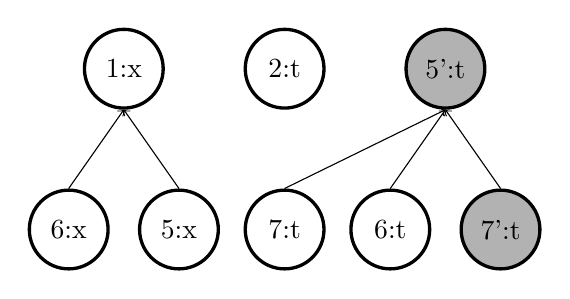
\begin{tikzpicture}[
source/.style={circle, draw=black, fill=white, very thick, minimum size=10mm},
synthesized/.style={circle, draw=black, fill=gray!60, very thick, minimum size=10mm}
]
\node[source](x_dec){1:x};
\node[source](tmp_dec)[right=of x_dec]{2:t};
\node[synthesized](tmp_dec_2)[right=of tmp_dec]{5':t};

\node[source](x_ref)[below=of x_dec,xshift=7mm]{5:x};
\node[source](x_ref_2)[below=of x_dec,xshift=-7mm]{6:x};
\node[source](tmp_ref)[below=of tmp_dec_2,xshift=-7mm]{6:t};
\node[synthesized](tmp_ref_2)[below=of tmp_dec_2,xshift=7mm]{7':t};

\node[source](tmp_ref_3)[below=of tmp_dec]{7:t};

\draw[->] (x_ref.north) -- (x_dec.south);
\draw[->] (x_ref_2.north) -- (x_dec.south);
\draw[->] (tmp_ref.north) -- (tmp_dec_2.south);
\draw[->] (tmp_ref_2.north) -- (tmp_dec_2.south);
\draw[->] (tmp_ref_3.north) -- (tmp_dec_2.south);
\end{tikzpicture}
\end{minipage}

\caption{Target program generated by swap language extension and corresponding name graph} \label{fig:name-graph}
\end{figure}

Node \textit{7:t} and \textit{6:t} originate from the source program but reference a synthesized declaration. Node \textit{5:t} shadows the original declaration \textit{2:t}. \textit{name-fix} adds node \textit{5:t} to the list of declarations to be renamed. After the entire name graph is analyzed/generated all declarations from this list are rebound under free names (i.e. names not yet bound in the target program). Since \textit{7:t} and \textit{6:t} are not correct references of \textit{5:t} they are not renamed. The resulting name graph and target program are presented in figure \ref{fig:name-graph-fixed}

\begin{figure}[h]
\centering
\begin{minipage}{0.25\linewidth}
\begin{lstlisting}
	var x = 0,
		tmp = 1;

	(function() {
		var tmp$0 = x;
		x = tmp;
		tmp = tmp$0;
	})();
\end{lstlisting}
\end{minipage}
\hfill
\begin{minipage}{0.65\linewidth}
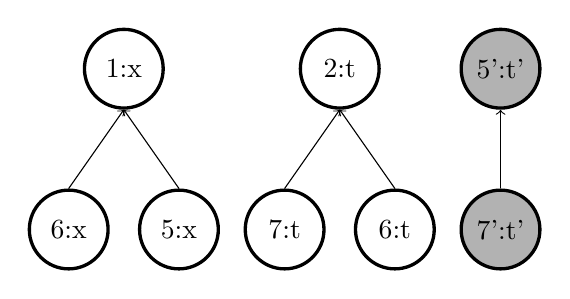
\begin{tikzpicture}[
source/.style={circle, draw=black, fill=white, very thick, minimum size=10mm},
synthesized/.style={circle, draw=black, fill=gray!60, very thick, minimum size=10mm}
]
\node[source](x_dec){1:x};
\node[source](tmp_dec)[right=of x_dec,xshift=7mm]{2:t};
\node[synthesized](tmp_dec_2)[right=of tmp_dec]{5':t'};

\node[source](x_ref)[below=of x_dec,xshift=7mm]{5:x};
\node[source](x_ref_2)[below=of x_dec,xshift=-7mm]{6:x};
\node[source](tmp_ref)[below=of tmp_dec,xshift=7mm]{6:t};
\node[synthesized](tmp_ref_2)[below=of tmp_dec_2]{7':t'};

\node[source](tmp_ref_3)[below=of tmp_dec,xshift=-7mm]{7:t};

\draw[->] (x_ref.north) -- (x_dec.south);
\draw[->] (x_ref_2.north) -- (x_dec.south);
\draw[->] (tmp_ref.north) -- (tmp_dec.south);
\draw[->] (tmp_ref_2.north) -- (tmp_dec_2.south);
\draw[->] (tmp_ref_3.north) -- (tmp_dec.south);
\end{tikzpicture}
\end{minipage}

\caption{Target program and name graph after \textit{name-fix} algorithm} \label{fig:name-graph-fixed}
\end{figure}

\textit{name-fix} does apply a \textit{"a closed-world assumption to infer that all unbound variables are indeed free, and thus can be renamed at will."}~\cite{Erdweg2014}. This means that global variables defined by the user (or a third-party library) that are included within the same run-time as our target program, could possibly be shadowed by the renamed bindings. However there is no way for \textit{name-fix} to know what bindings will be taken by other bindings than those bound in the source program.

\paragraph{Combined language extensions} \label{par:combined-extensions}
Language extensions can depend upon other language extensions to work correctly, this dependency makes a collection of language extensions less modular because the depended extension always needs to be used in combination with it's dependency. It would be preferable if the two extensions could be used in separation where functionality which relies on both extensions working together is only enabled in a situation where the two language extensions are used.

An example of such overlapping functionality in the ES 6 specification is that of destructuring assignment (see appendix \ref{destructuring}) inside for-of loops (see appendix \ref{for-of}).

\begin{lstlisting}
for(var [a,b] of [ [1,2], [3,4] ]) {
	// ... do something with a and b
}
\end{lstlisting}

The for-of loop needs a dependency on the destructuring assignment syntax definition, to be able to create the statement syntax to allow an assignment pattern (i.e. either an array or object destructuring) inside the for-of loop:

\begin{lstlisting}
syntax Statement
	= "for" "(" "var" AssignmentPattern "of" Expression ")" Statement;
\end{lstlisting}

Shared language extensions need to have a non-terminal defined in the base-language which can be extended in both language extensions. In case of the for-of loop we can introduce a new non-terminal \textit{ForBinding} which can be extended in the destructuring assignment language extension.

\begin{lstlisting}
// Core syntax definition
syntax ForBinding
	= Id;

// For-of loop language extension
syntax Statement
	= "for" "(" "var" ForBinding "of" Expression ")" Statement;

// Destructuring language extension
syntax ForBinding
	= AssignmentPattern;
\end{lstlisting}

Designing language extensions in this way makes the entire suite of language extensions more modular, because we can combine language extensions that depend on each other for full functionality. Or use them separately to get only their independent functionality.

% Chapter Template

\chapter{Results and Comparison} % Main chapter title

\label{Chapter4}

\lhead{Chapter 4. \emph{Results and Comparison}}

\section{Evaluation}

There are several criteria as to which we evaluate the resulting transformation suite. These criteria are described in the following table.

\begin{table}[h]
\def\arraystretch{1.5}
\caption{Evaluation criteria}
\label{criteria}
\begin{tabular}{rp{0.7\linewidth}}
{\bf Correctness} & A language extension is performed correct if the target program is semantically similar to that of the language feature defined in the ECMAScript 6 specification\cite{SpecJS}. To test the correctness we use a test-suite created especially for this purpose\footnotemark\\
{\bf Modularity}  & Is it possible separate and recombine the different language extensions.\\
{\bf Size}        & How many lines of code are used to implement the transformation suite, if possible compared on a feature basis\\
{\bf Output "noise"} & One of the challenges programmers face when using program transformations is the debugging of the generated program. During transformation the language extensions are eliminated from their code (and replaced by core language constructs). The more "noise" a transformation (suite) generates the harder it becomes for a programmer to debug generated code. An informal definition of noise is code added by a transformation that removes structure of the target program further away from the source program. \\
{\bf Coverage}    & How many language features are implemented\\
{\bf Performance} & What is the run time of the transformation code\\
\end{tabular}
\end{table}
\footnotetext{\url{https://kangax.github.io/compat-table/es6/}}

To evaluate our implementation of the transformation suite we validate against three open-source implementation of ECMAScript 6 language as a transformation suite (to ECMAScript 5). We selected the following \textit{transpilers} (these transformation suites categories themselves as transpilers a combination of compiler and transformer) to evaluate against:

\begin{table}[h]
\def\arraystretch{1.5}
\caption{Open-source ES6 transpilers}
\label{transpilers}
\begin{tabular}{rp{0.5\linewidth}p{0.1\linewidth}p{0.1\linewidth}}
 & \textbf{Description} & \textbf{Cont.} & \textbf{Com.} \\
{\bf Babel JS\footnotemark[1]} & The most used ECMAScript 6 to 5 transpiler (was named 6to5 before). It is created using JavaScript and relies on the Acorn\footnotemark[4] JavaScript parser. & 105 & 4582 \\
{\bf Traceur\footnotemark[2]} & This transpiler is produced by a team from Google. Written in JavaScript and includes its own parser. This transpiler relies more heavily on a run-time environment than the other transpilers. & 55 & 1584\\
{\bf ES6-Transpiler\footnotemark[3]} & Apart form Traceur and Babel JS there only exist small individual projects that implement ES6 to 5 transpilers. This is the most feature complete of those transpilers. It relies on the ESPrima\footnotemark[5] JavaScript parser. & 5 & 250 \\
\end{tabular}
\end{table}
\footnotetext[1]{\url{http://www.babeljs.io}}
\footnotetext[2]{\url{https://github.com/google/traceur-compiler}}
\footnotetext[3]{\url{https://github.com/termi/es6-transpiler}}
\footnotetext[4]{\url{https://github.com/marijnh/acorn}}
\footnotetext[5]{\url{http://esprima.org/}}

\paragraph{Correctness} \label{sec:correctness}
In table \ref{tab:compatibility} results of the compatibility tests. Four categories are of interest because they provide tests for the new language features of ES 6, and not tests for new standard-library functionality introduced by ES 6. Syntax depicts the category testing all language features that introduce new syntactical elements. Tests regarding the new binding mechanisms fall under the category Bindings. Tests for the new function types (i.e. generators, arrow functions, and classes) fall under the Function category. 

Not all tests can be satisfied by a transformation suite alone, some tests use the \textit{eval} function to evaluate a string as JavaScript in the current run-time. A transformation suite only has access to the static semantics during transformation it can not resolve the \textit{string} that is going to be evaluated during run-time. Because other transformation suites face the same issue we do not remove these tests from the set of tests. 

Our implementation does not score as high as the big open-source projects, mainly because we do not implement generators and automatically fail twenty-two tests related to generators. ES6-transpiler scores lower than our implementation. The compatibility score indicates that our artifact could be used in a \textit{real-world} environment, as long as unimplemented features are avoided. For a full list of features implemented by our artifact consult appendix \ref{AppendixA}.

\begin{table}[h]
\centering
\caption{Compatibility tests} \label{tab:compatibility}
\begin{tabular}{@{}lccccc@{}}
\toprule
                & {\bf Total} & \multicolumn{1}{l}{{\bf Babel}} & \multicolumn{1}{l}{{\bf Traceur}} & \multicolumn{1}{l}{{\bf ES6 Transpiler}} & \multicolumn{1}{l}{{\bf Rascal}} \\ \midrule
{\bf Syntax}    & 76          & 76                              & 60                     & 46           & 64                               \\
{\bf Bindings}  & 19          & 15                              & 15                     & 10           & 16                               \\
{\bf Functions} & 62          & 54                              & 50                     & 43           & 35                               \\
{\bf Total}     & 157         & 136 (87\%)                      & 125 (80\%)             & 99 (63\%)    & 115 (73\%)                        \\ \bottomrule
\end{tabular}
\end{table}

\paragraph{Modularity}

\paragraph{Size}
In table \ref{tab:loc} we compare the size of all projects in lines of code, where our own artifact is named Rascal. Lines of code are measured using the \textit{cloc} tool\footnote{\url{http://cloc.sourceforge.net/}}, because \textit{cloc} has no built in support to measure lines of code of Rascal programs we forced \textit{cloc} to measure Rascal programs as if they where \textit{Java} code (Rascal comments are similar to those of Java).

Our artifact is about five times smaller in size, compared to other implementations. 

Our artifact relies on the Rascal parser generator and a Rascal syntax definition to define the ES 5 grammar, and ES 6 language extensions. Other implementations rely on open-source ECMAScript parsers implemented in JavaScript, or implement their own parser. The syntax definitions are about eight to ten times smaller in size than any of the JavaScript parsers. Rascal syntax definitions do impose some limitations that made it difficult or impossible to implement certain language grammar features, in appendix \ref{AppendixA} we elaborate on this.

\begin{table}[h]
\caption{Lines of code - transformations \& parser} \label{tab:loc}
\begin{minipage}{0.45\linewidth}
\begin{tabular}{@{}lrr@{}}
\toprule
              & {\bf Files} & \multicolumn{1}{l}{{\bf Lines of code}} \\ \midrule
{\bf Babel}   & 76          & 6547                                    \\
{\bf Traceur} & 19          & 9881                                    \\
{\bf ES6 Transpiler} & 22    & 5341
\\
{\bf Rascal}  & 62          & 1368                                    \\ \bottomrule
\end{tabular}
\end{minipage}
\hfill
\begin{minipage}{0.45\linewidth}
\begin{tabular}{@{}lrr@{}}
\toprule
              & {\bf Files} & \multicolumn{1}{l}{{\bf Lines of code}} \\ \midrule
{\bf Acorn}   & 22          & 3583                                    \\
{\bf Traceur} & 15          & 6681                                    \\
{\bf ESprima} & 1           & 4323
\\
{\bf Rascal}  & 12          & 555                                    \\ \bottomrule
\end{tabular}
\end{minipage}
\end{table}

In table \ref{tab:loc-feature} we analyze the size of each transpiler on a feature basis, where only the size of actual transformation code for an extension is measured. Rascal's implementation and that of Babel JS have simlilar sizes for transformations. Traceur and ES6 transpiler's size difference as compared to Rascal's implementation are similar to that of the size different of the projects as a whole. 

The main reason why Babel JS is able to reduce the size of their transformations is because of the architecture of the project. Many concerns are extracted from transformation code and solved separately in different modules/files. Some examples: creating new bindings (\textit{src/babel/traversal/scope/binding.js}), pattern matching on parse tree nodes (\textit{src/babel/traversal} LOC: 2456), creating new abstract syntax (\textit{src/babel/transformations/templates} LOC: 456). 

\begin{table}[h]
\centering
\caption{BabelJS - Lines of code per transformation} \label{tab:loc-feature}
\begin{tabular}{@{}lrrrr@{}}
\toprule
                           & \textbf{Babel JS} & \textbf{Traceur} & \textbf{ES6 transpiler} & \textbf{Rascal} \\ \midrule
\textbf{Arrow functions}   & 7                 & 144              & 277\footnotemark[1]     & 40 \\
\textbf{Classes}           & 390               & 286              & 498                     & 215 \\
\textbf{Destructuring}     & 349               & 403              & 303                     & 261 \\
\textbf{For of loop}       & 127               & 90               & 529                     & 159 \\
\textbf{Binding}           & 513               & 651              & 219                     & 221 \\
\textbf{Parameters}        & 192               & 554              & 277\footnotemark[1]     & 58 \\
\textbf{Object literals}   & 74                & 248              & 204                     & 74 \\
\textbf{Spread}            & 93                & 117              & 460                     & 57 \\
\textbf{Template literals} & 64                & 203              & -\footnotemark          & 89 \\
\textbf{Numeric literals}  & -                 & 31               & 22                      & - \\ \bottomrule
\end{tabular}
\end{table}
\footnotetext[1]{ES6 transpiler does not have separate files for arrow function and paramater transformation, these both reside in \textit{functions.js}. This number is the size (in lines of code) of this file.}
\footnotetext{Not implemented by ES6 transpiler}

\paragraph{Noise}

\paragraph{Coverage}

\paragraph{Performance}

\section{Related Work}
Eelco Visser,
name-fix algo,
Irvine program transformation catalog,
Maerds

 
%\chapter{Implementation \projectname} % Main chapter title

\label{Chapter5}

\lhead{Chapter 5. \emph{Implementation} {\projectname}}

Each transformation is defined as one or more rewrite rules. It has a concrete syntax pattern which matches part of a parse-tree. The result is a concrete piece of syntax, using only constructs from the core syntax definition (i.e. ES 5).
The rewrite rules are exhaustively applied on the input parse-tree until no more rewrite rules match any sub-trees of the input. Application of rewrite rules to the parse-tree is done bottom-up because several rewrite rules (e.g. arrow function) demand their sub-terms to be transformed to guarantee successful completion.

\section{Basics}
To get a better understanding of the inner working of \projectname we discuss the implementation of the \lstinline$swap$ language extension (see section \ref{hygiene}). The language extension introduces a new statement 

\begin{lstlisting}[caption=Core syntax,language=rascal]
module core::Syntax

syntax Statement 
	= ...
	| ...
	...;
\end{lstlisting}

To extend the list of possible statements we create a new Rascal module that extends the core syntax definition and defines a new syntax rule for \textit{Statement} named \textit{swap}. With this new syntax rule our parser is able to correctly parse \lstinline$swap$ statements.

\begin{lstlisting}[caption=Swap statement syntax,language=rascal]
extends core::Syntax;

syntax Statement = swap: "swap" Id Id ";";
\end{lstlisting}

Before we create a function that transforms the \lstinline$swap$ statement to JavaScript code we introduce a simple visitor and default desugar function. A default desugar function for statements is defined which is the id function on a statement. To desugar an entire parse tree we only have to visit each node (bottom up) and invoke the desugar function for each statement that is found by the visitor.

\begin{lstlisting}[caption=Desugar visitor, language=rascal]
default Statement desugar( Statement s ) = s;

Source runDesugar( Source pt ) {
	return visit(pt) {
		case Statement s => desugar(s)
	}
}
\end{lstlisting}

To desugar the new syntax construct to JavaScript code we overload the previously defined desugar function with a pattern match on 
\textit{Statement} to match the use of the \lstinline$swap$ statement and translate it to an immediately invoking function expression (IIFE) in which we rebind both supplied identifiers to each other.

% \CAT{Keyword}{syntax} Statement = \CAT{Constant}{"swap"} Id Id;

\begin{rascal}
Statement desugar( (Statement)`\CAT{Keyword}{swap} \CAT{MetaVariable}{\textless{}Id x\textgreater{}} \CAT{MetaVariable}{\textless{}Id y\textgreater{}}` )
    = (Statement)
            `(\CAT{Keyword}{function}() \{{}
            	\CAT{Keyword}{var} tmp = \CAT{MetaVariable}{\textless{}Id x\textgreater{}};
            	\CAT{MetaVariable}{\textless{}Id x\textgreater{}} = \CAT{MetaVariable}{\textless{}Id y\textgreater{}};
            	\CAT{MetaVariable}{\textless{}Id y\textgreater{}} = tmp;
            \}{})();`;
\end{rascal}

The argument of desugar is a pattern match on parse-tree nodes of the type \lstinline$Statement$ matching on \lstinline$swap$ statements, if a match is found the identifiers supplied to the statement are bound respectively to \lstinline$x$ and \lstinline$y$. The function returns a piece of concrete syntax which in turn is of the type \lstinline$Statement$ where the supplied identifiers are rebound to each other. Remember that the supplied identifiers to the \lstinline$swap$ statement could have any name, what would happen if one of the identifiers was name \lstinline$tmp$?

\section{\projectname}
In \textit{\projectname} we implement a large subset of ES6 features as language extensions on top of a core syntax describing ES5. Here we discuss several parts of interest from our implementation. Everything with the exception of let-const is based on the simple example described in the previous section. 

\subsection{Visitor}
In our basic example we used a function \lstinline$runDesugar$, this is the visitor of the parse-tree and is in principle how the visitor of {\projectname} works. Differences are we also match on expressions, functions, and the source node (root node) this final match can be used by transformations that are performed global-to-local or global-to-global. If we have multiple language extensions performing a global-to-local or global-to-global transformation or if a language extension's transformation introduces a language construct that should be desugared either by itself or another language extension, one pass over the parse tree is not enough. For extensions with these kind of transformations we need to revisit the tree until no more changes are applied by desugar functions. The final desugar visitor and default desugar functions are as follows, where \textit{solve} will ensure we revisit the tree until no more desugarings are performed:

\begin{lstlisting}[caption=Identity desugar functions, language=rascal]
default Source desugar( Source s ) = s;
default Function desugar( Function s ) = s;
default Statement desugar( Statement s ) = s;
default Expression desugar( Expression s ) = s;
\end{lstlisting}

\begin{lstlisting}[caption=Final desugar visitor, language=rascal]
Source runDesugar( Source pt ) {
	return solve(pt) {
		pt = visit(pt) {
			case Source src => desugar(src)
			case Function f => desugar(f)
			case Statement s => desugar(s)
			case Expression e => desugar(e)
		}
	}
}
\end{lstlisting}

An example of a language extension that relies on a global-to-local transformation is the arrow function. Arrow function's that reside directly in the global scope, are desugared differently from locally defined arrow functions. See appendix \ref{arrow}

\subsection{Introducing bindings}
Some language extensions need to introduce new bindings in the target program to work properly. There are multiple ways for a transformation to introduce bindings in JavaScript. When a transformation is performed on an expression an IIFE can be used to introduce new bindings only accesible in the scope of this expression.

\begin{minipage}{0.45\linewidth}
\begin{lstlisting}
<Expression e>
\end{lstlisting}
\end{minipage}
\hfill
\begin{minipage}{0.45\linewidth}
\begin{lstlisting}
(function(x, y, ...) {
	return <Expression e>;
})(xd, yd, ...)
\end{lstlisting}
\end{minipage}

When a transformation is performed on a statement a block statement can be used in combination with variables declared through the \textit{let} declarator, to introduce variables only accessible in the scope of the statement. \textit{Let} declarations are however not part of ES5 JavaScript but introduced by ES6, this assumes there is a language extension for \textit{let} present (see appendix \ref{let-const}).

\begin{minipage}{0.45\linewidth}
\begin{lstlisting}
<Statement s>
\end{lstlisting}
\end{minipage}
\hfill
\begin{minipage}{0.45\linewidth}
\begin{lstlisting}
{
	let x = xd,
		y = yd
		...;
	<Statement s>
}
\end{lstlisting}
\end{minipage}

In the case of a statement an IIFE can not be used to introduce new bindings because the control flow of the target program would break if the desugared statement contains a non-local control flow construct, such as \lstinline$return$ or \lstinline$break$. 

\subsection{Mutually dependent language extensions} \label{par:combined-extensions}
Language extensions can depend upon other language extensions to work correctly, this dependency makes a collection of language extensions less modular because the dependent extension always needs to be used in combination with its dependency. It would be preferable if the two extensions could be used in separation where functionality which relies on both extensions working together is only enabled in a situation where the two language extensions are used.

An example of language extension with mutually dependent functionality in the ES 6 specification is that of destructuring assignment (see appendix \ref{destructuring}) inside for-of loops (see appendix \ref{for-of}).

\begin{lstlisting}
for(var [a,b] of [ [1,2], [3,4] ]) {
	// ... do something with a and b
}
\end{lstlisting}

The for-of loop needs a dependency on the destructuring assignment syntax definition, to be able to create the statement syntax to allow an assignment pattern (i.e. either an array or object destructuring) inside the for-of loop:

\begin{lstlisting}[language=rascal]
syntax Statement
	= "for" "(" "var" AssignmentPattern "of" Expression ")" Statement;
\end{lstlisting}

Shared language extensions need to have a non-terminal defined in the base-language which can be extended in both language extensions. In case of the for-of loop we can introduce a new non-terminal \textit{ForBinding} which can be extended in the destructuring assignment language extension.

\begin{lstlisting}[language=rascal]
// Core syntax definition
syntax ForBinding
	= Id;

// For-of loop language extension
syntax Statement
	= "for" "(" "var" ForBinding "of" Expression ")" Statement;

// Destructuring language extension
syntax ForBinding
	= AssignmentPattern;
\end{lstlisting}

How are the transformations of both extensions affected by the fact that they are mutually dependent on each other? Before this question can be answered we need insight in how a \textit{for-of} loop is desugared, this is explained in appendix \ref{for-of}. For this example we just assume a \textit{for-of} loop is desugared to a traditional \textit{for} loop over the length property of the input array (ignoring some of the intricacies of \textit{for-of} loop language extension). The following example presents the wanted desugaring where the assignment pattern binding is moved to the body of the loop. 

\begin{minipage}{0.45\linewidth}
\begin{lstlisting}
for(var [a,b] of arr) {
	<Statement* body>
}
\end{lstlisting}
\end{minipage}
\hfill
\begin{minipage}{0.5\linewidth}
\begin{lstlisting}
for(var i = 0; i < arr.length; i++) 
{	
	var [a,b] = arr[i];
	<Statement* body>
}
\end{lstlisting}
\end{minipage}

The complexity in the desugar function of a \textit{for-of} loop lies in the fact that the \lstinline$ForBinding$ non-terminal can consist either of an \lstinline$Identifier$ or an \lstinline$AssignmentPattern$ non-terminal. The \textit{for-of} loop language extension is however unaware of the existence of the second option, because it is created by the \textit{destructuring} language extension, and thus unable to correctly desugar in this case. To solve this issue we introduce a function that can be overloaded in the \textit{destructuring} language extension to help transform the \lstinline$ForBinding$ to a \lstinline$VariableDeclaration$, this function is named \textit{declareBinding}.

\begin{lstlisting}[caption=default \textit{declareBinding} function from \textit{for-of} language extension,language=rascal]
VariableDeclaration declareBinding( (ForBinding)`<Id id>`, Expression e )
	= (VariableDeclaration)`<Id id> = <Expression e>`;
\end{lstlisting}

\begin{lstlisting}[caption=overloaded \textit{declareBinding} function from \textit{destructuring} language extension,language=rascal]
VariableDeclaration declareBinding( (ForBinding)`<AssignmentPattern p>`, Expression e )
	= (VariableDeclaration)`<AssignmentPattern p> = <Expression e>`;
\end{lstlisting}

Designing language extensions in this way makes the entire suite of language extensions more modular. Language extensions can be mutually dependent instead of having explicit dependencies on one another. This presents the possibility of selecting only the needed language extensions without being required to depend on unneeded language extensions. And at the same time it reduces the amount of code needed for the implementation of language extensions that are mutually dependent. In case of our example above if we had an explicit dependency from \textit{destructuring} to \textit{for-of} the desugaring function for \textit{for-of} loops had to be overridden in the \textit{destructuring} language extension.

\subsection{Variable capture}
In section \ref{hygiene} we have described the problem of variable capture in the context of program transformations. 
Here we discuss the algorithm reused to solve variable capture in \projectname, the algorithm reused is named \textit{\vfix}. The algorithm relies on a binding graph to identify variable capture, and uses string origins~\cite{Inostroza2014} to distinguish between synthesized identifiers (i.e. those identifiers introduced by the transformation) and identifiers originating from the source program.

\textit{\vfix} analyses the \textit{name graph} of generated program to identify variable capture. The name graph contains nodes for all identifiers in the program, a directed edge indicates a reference to a declaration. Because our source and target language are both JavaScript and thus have the same binding mechanism, we only generate the name graph for our target program. In the graph a distinction is made between synthesized and user bindings. To identify whether a binding originates from the source program or was synthesized during transformation, the \textit{\vfix} algorithm uses origin tracking~\cite{Inostroza2014} to identify the origin of identifier (either from the source program or introduced by a transformation).

In figure \ref{fig:name-graph} we use the target program from our \lstinline$swap$ language extension (see section \ref{hygiene}) to illustrate how these name graphs are constructed, and how \textit{\vfix} identifies variable capture. Each node contains a line number and the identifier it resembles from that line, a directed edge is a reference to a declaration. Nodes with a white background originate from the source program, nodes with a dark background are synthesized during transformation. Line numbers from synthesized identifiers are appended with a tick.

\begin{figure}[h]
\centering
\begin{minipage}{0.25\linewidth}
\begin{lstlisting}
	var x = 0,
		tmp = 1;

	(function() {
		var tmp = x;
		x = tmp;
		tmp = tmp;
	})();
\end{lstlisting}
\end{minipage}
\hfill
\begin{minipage}{0.65\linewidth}
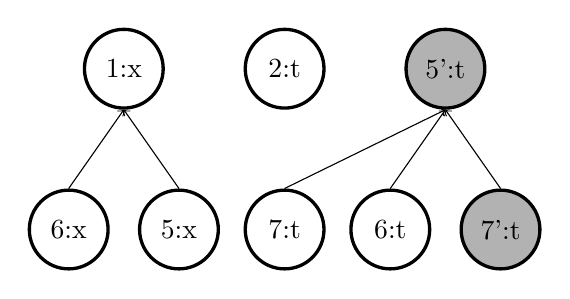
\begin{tikzpicture}[
source/.style={circle, draw=black, fill=white, very thick, minimum size=10mm},
synthesized/.style={circle, draw=black, fill=gray!60, very thick, minimum size=10mm}
]
\node[source](x_dec){1:x};
\node[source](tmp_dec)[right=of x_dec]{2:t};
\node[synthesized](tmp_dec_2)[right=of tmp_dec]{5':t};

\node[source](x_ref)[below=of x_dec,xshift=7mm]{5:x};
\node[source](x_ref_2)[below=of x_dec,xshift=-7mm]{6:x};
\node[source](tmp_ref)[below=of tmp_dec_2,xshift=-7mm]{6:t};
\node[synthesized](tmp_ref_2)[below=of tmp_dec_2,xshift=7mm]{7':t};

\node[source](tmp_ref_3)[below=of tmp_dec]{7:t};

\draw[->] (x_ref.north) -- (x_dec.south);
\draw[->] (x_ref_2.north) -- (x_dec.south);
\draw[->] (tmp_ref.north) -- (tmp_dec_2.south);
\draw[->] (tmp_ref_2.north) -- (tmp_dec_2.south);
\draw[->] (tmp_ref_3.north) -- (tmp_dec_2.south);
\end{tikzpicture}
\end{minipage}

\caption{Target program generated by swap language extension and corresponding name graph; where \textit{t} stands for \textit{tmp}} \label{fig:name-graph}
\end{figure}

Node \textit{7:tmp} and \textit{6:tmp} originate from the source program but reference a synthesized declaration. Node \textit{5:tmp} shadows the original declaration \textit{2:tmp}. \textit{\vfix} adds node \textit{5:tmp} to the list of declarations to be renamed. After the entire name graph is analyzed/generated all declarations from this list are renamed to free names (i.e. names not yet bound in the target program). Since \textit{7:tmp} and \textit{6:tmp} are not correct references of \textit{5:tmp} they are not renamed. The resulting name graph and target program are presented in figure \ref{fig:name-graph-fixed}

\begin{figure}[h]
\centering
\begin{minipage}{0.25\linewidth}
\begin{lstlisting}
	var x = 0,
		tmp = 1;

	(function() {
		var tmp$0 = x;
		x = tmp;
		tmp = tmp$0;
	})();
\end{lstlisting}
\end{minipage}
\hfill
\begin{minipage}{0.65\linewidth}
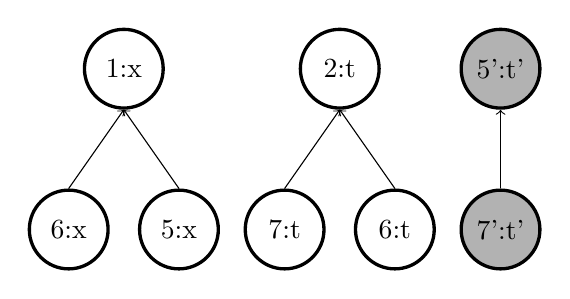
\begin{tikzpicture}[
source/.style={circle, draw=black, fill=white, very thick, minimum size=10mm},
synthesized/.style={circle, draw=black, fill=gray!60, very thick, minimum size=10mm}
]
\node[source](x_dec){1:x};
\node[source](tmp_dec)[right=of x_dec,xshift=7mm]{2:t};
\node[synthesized](tmp_dec_2)[right=of tmp_dec]{5':t'};

\node[source](x_ref)[below=of x_dec,xshift=7mm]{5:x};
\node[source](x_ref_2)[below=of x_dec,xshift=-7mm]{6:x};
\node[source](tmp_ref)[below=of tmp_dec,xshift=7mm]{6:t};
\node[synthesized](tmp_ref_2)[below=of tmp_dec_2]{7':t'};

\node[source](tmp_ref_3)[below=of tmp_dec,xshift=-7mm]{7:t};

\draw[->] (x_ref.north) -- (x_dec.south);
\draw[->] (x_ref_2.north) -- (x_dec.south);
\draw[->] (tmp_ref.north) -- (tmp_dec.south);
\draw[->] (tmp_ref_2.north) -- (tmp_dec_2.south);
\draw[->] (tmp_ref_3.north) -- (tmp_dec.south);
\end{tikzpicture}
\end{minipage}

\caption{Target program and name graph after \textit{\vfix} algorithm; where \textit{t} stands for \textit{tmp} and \textit{t'} for \textit{tmp\$0}} \label{fig:name-graph-fixed}
\end{figure}

\textit{\vfix} does apply a \textit{``closed-world assumption to infer that all unbound variables are indeed free, and thus can be renamed at will.''}~\cite{Erdweg2014}. This means that global variables defined by the user (or a third-party library) that are included within the same run-time as our target program, could possibly be shadowed by the renamed bindings. However there is no way for \textit{\vfix} to know what names will be taken by other bindings than those bound in the source program.

A second form of variable capture is introduced when the user shadows a global variable on which a target program relies. \textit{\vfix} is also able to solve this form of variable capture, to illustrate this we use the example of the \lstinline$log$ language extension. The name-graph for the target program of our example (see section \ref{hygiene}) shows a reference from an identifier introduced by our transformation to a source binding (see figure \ref{fig:vfix2}).

\begin{figure}[h]
\centering
\begin{minipage}{0.65\linewidth}
\begin{lstlisting}
	var console = <Expression e>;
	console.log("message");
	console;
\end{lstlisting}
\end{minipage}
\hfill
\begin{minipage}{0.25\linewidth}
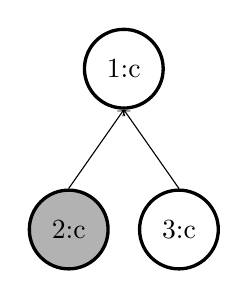
\begin{tikzpicture}[
source/.style={circle, draw=black, fill=white, very thick, minimum size=10mm},
synthesized/.style={circle, draw=black, fill=gray!60, very thick, minimum size=10mm}
]
\node[source](console_dec){1:c};

\node[synthesized](console_ref)[below=of console_dec,xshift=-7mm]{2:c};
\node[source](console_ref_2)[below=of console_dec,xshift=7mm]{3:c};

\draw[->] (console_ref.north) -- (console_dec.south);
\draw[->] (console_ref_2.north) -- (console_dec.south);
\end{tikzpicture}
\end{minipage}
\caption{Target program generated by log language extension and corresponding name-graph; where \textit{c} stands for \textit{console}} \label{fig:vfix2}
\end{figure}

This reference is identified as variable capture and declaration \lstinline$console$ is marked to be renamed (see figure \ref{fig:vfix2}. 

\begin{figure}[h]
\centering
\begin{minipage}{0.65\linewidth}
\begin{lstlisting}
	var console$0 = <Expression e>;
	console.log("message");
	console$0;
\end{lstlisting}
\end{minipage}
\hfill
\begin{minipage}{0.25\linewidth}
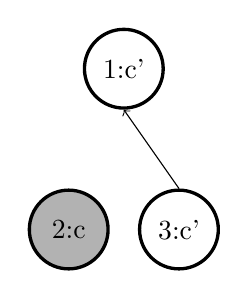
\begin{tikzpicture}[
source/.style={circle, draw=black, fill=white, very thick, minimum size=10mm},
synthesized/.style={circle, draw=black, fill=gray!60, very thick, minimum size=10mm}
]
\node[source](console_dec){1:c'};

\node[synthesized](console_ref)[below=of console_dec,xshift=-7mm]{2:c};
\node[source](console_ref_2)[below=of console_dec,xshift=7mm]{3:c'};

\draw[->] (console_ref_2.north) -- (console_dec.south);
\end{tikzpicture}
\end{minipage}
\caption{Target program and name-graph after application of \textit{\vfix} algorithm; where \textit{c} stands for \textit{console} and \textit{c'} for \textit{console\$0}} \label{fig:vfix2_fixed}
\end{figure}

Notice that the \textit{\vfix} algorithm in the example of the \lstinline$swap$ language extension (see figure \ref{fig:name-graph-fixed}) renames a synthesized binding. Whereas in case of the \lstinline$log$ language extension (see figure \ref{fig:vfix2_fixed}) the \textit{\vfix} algorithm renames an identifier originating from the source program. When identifiers from the source program are renamed external scripts relying on these bindings will no longer function correctly.

\subsection{Block scoping}

As described in section \ref{javascript-scoping} JavaScript's bindings are function scoped, i.e. they are accessible throughout the entire lexical scope of the function they are defined in. ES6 introduces a new binding mechanism through which identifiers can be bound in a block scope (see appendix \ref{let-const}). Block bound identifiers are only available after declaration within the lexical enclosing block scope they are defined in. Where normal declarations can be redeclared without errors, redeclration of block bound bindings is illegal and results in a parse error. To desugar the new block binding introduced in ES6  there are two approaches. First, replace all block binding by a \textit{try catch} block where we throw the binding inside of the try block and catch the binding in the catch block.

\begin{minipage}{0.45\linewidth}
\begin{lstlisting}
let x = 0;
... statements
\end{lstlisting}
\end{minipage}
\hfill
\begin{minipage}{0.45\linewidth}
\begin{lstlisting}
try {
	throw 0;
} catch(x) {
	... statements
}
\end{lstlisting}
\end{minipage}

The problem with this implementation is that \textit{try catch} blocks are not optimized by interpreters\footnote{\url{http://ryanmorr.com/reinventing-the-try-catch-block/}} and thus the performance of transformed code would be much worse than that of the source program. Second, the block binding could be achieved through the renaming of bindings to avoid reference of \textit{let} or \textit{const} defined bindings outside of their block scope.

\begin{minipage}{0.45\linewidth}
\begin{lstlisting}
{
	let x = 0;
	x;
}
x;
\end{lstlisting}
\end{minipage}
\hfill
\begin{minipage}{0.45\linewidth}
\begin{lstlisting}
{
	var x_0 = 0;
	x_0;
}
x;
\end{lstlisting}
\end{minipage}

To resolve the naming needed for the emulation of block scope in ES5 we also use a \textit{name-graph} as described in the previous section. To identify illegal references in the name graph we compare a name graph with block binding against a name graph without block binding, the two graphs for the example are depicted below.

\begin{figure}
\begin{subfigure}{.45\textwidth}
\centering
\resizebox{0.4\linewidth}{!}{
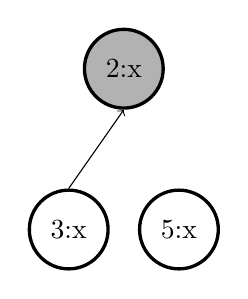
\begin{tikzpicture}[
source/.style={circle, draw=black, fill=white, very thick, minimum size=10mm},
synthesized/.style={circle, draw=black, fill=gray!60, very thick, minimum size=10mm}
]
\node[synthesized](x_dec)[align=center]{2:x};

\node[source](x_ref)[below=of x_dec,xshift=-7mm]{3:x};
\node[source](x_ref_2)[below=of x_dec,xshift=7mm]{5:x};

\draw[->] (x_ref.north) -- (x_dec.south);
\end{tikzpicture}
}
\subcaption{Name graph (block scope binding)}
\end{subfigure}
\hfill
\begin{subfigure}{.45\textwidth}
\centering
\resizebox{0.4\linewidth}{!}{
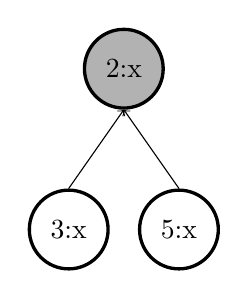
\begin{tikzpicture}[
source/.style={circle, draw=black, fill=white, very thick, minimum size=10mm},
synthesized/.style={circle, draw=black, fill=gray!60, very thick, minimum size=10mm}
]
\node[synthesized](x_dec){2:x};

\node[source](x_ref)[below=of x_dec,xshift=-7mm]{3:x};
\node[source](x_ref_2)[below=of x_dec,xshift=7mm]{5:x};

\draw[->] (x_ref.north) -- (x_dec.south);
\draw[->] (x_ref_2.north) -- (x_dec.south);
\end{tikzpicture}
}
\subcaption{Name graph (function scope binding)}
\end{subfigure}
\end{figure}

The first name graph is the one created using a block binding mechanism where \textit{const} and \textit{let} declarations are block bound. In the second name graph all declarations are bound in their lexical enclosing function's scope. Now we identify the reference from \textit{5:x} to the declaration \textit{2:x} as illegal, because it exists in our function scoped name graph but does not occur in the block bound name graph. Declaration \textit{2:x} is marked to be renamed. After the entire name graph is build and all illegal references are identified, all declarations and their references according to the block bound name graph are renamed.

\paragraph{Implementation}
For the implementation of the block binding resolver we use a special type of scope graph, consisting of three types of nodes. First, a root node created for the root (or global) scope of an input parse tree. This node contains an environment consisting of names with the location of their declaration. Second, each function scope is identified by a closure node. This node consists of an \lstinline$Env$ containing all function scoped definitions (i.e. declarations of functions or using \lstinline$var$ declarator). It also contains a \lstinline$LEnv$ which is the name-graph created where all bindings are function scoped (i.e. also declarations using \lstinline$let$ or \lstinline$const$ declarators). Third, a node block is created for each block of statements, containing all block-scoped declarations in an environment.

\begin{lstlisting}[caption=Data structure for scope graph,language=rascal]
alias LEnv = lrel[str name, loc def];
alias Env = map[str name,loc def];

data Scope 
	= block( Env environment, Scope parent )
	| closure( Env environment, LEnv closureEnvironment, Scope parent )
	| root( Env environment );
\end{lstlisting}

A resolver visits the parse-tree while building a scope trees for the current path. All declaration in a function's scope are hoisted, because these declarations can be referenced throughout the entire lexical scope of the function, even before their actual declaration. Usage of an identifier by reference are resolved through a function named \lstinline$lookup$:

\begin{lstlisting}[language=rascal]
set[loc] lookup(str name, loc use, Scope scope);
\end{lstlisting}

This function visits the scope tree (top-down, the root of the tree is the current scope). For block and root nodes the location of declaration of the binding is returned if it is present in the environment of that scope. If no declaration is found in block scopes and we visit a closure node we first identify whether any \textit{illegal} references are possible to declarations in other block scopes not accesible from our scope. Then we lookup whether a declaration exists in the current closure and return this declaration if it exists.

To detect illegal redeclarations a function name \lstinline$declare$ is called on each declaration. It checks whether the name is already declared in the current block-scope, in this case it sets an error message. If the binding is not yet declared in the block-scope it checks whether it is set in any other block-scopes of the current closure, in this case the declaration is marked for renaming.

\begin{lstlisting}[language=rascal]
bool declare(loc decl, str name, loc def, Scope scope);
\end{lstlisting}

\subsection{IDE integration}
Because the features described in the previous two sections need name graph analysis we can perform some static analysis on these graphs and integrate the resulting data with the IDE. First, the name graph gives us information of all references in the source file, with this information we create hyperlinks from references to declarations. Second, we can also identify a reference to an undefined binding and mark this reference with an error inside the IDE. Finally, bindings created by let (or const) are not allowed to be re-declared in the same scope, illegal redeclarations can be identified and marked with an error in the IDE.

\begin{figure}
\centering

\begin{subfigure}{.49\textwidth}
	\centering
	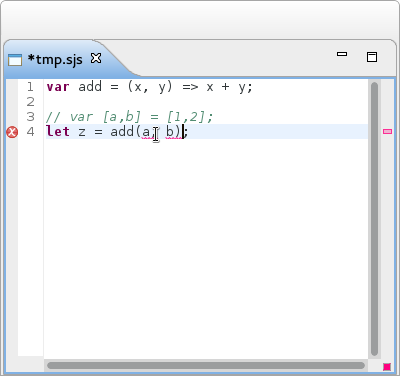
\includegraphics[width=\textwidth]{undeclared.png}
	\subcaption{Reference of undeclared bindings}
\end{subfigure}\hfill%
\begin{subfigure}{.49\textwidth}
	\centering	
	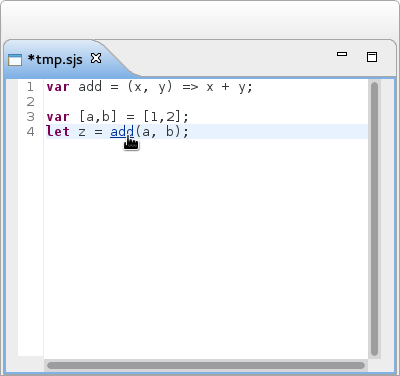
\includegraphics[width=\textwidth]{declared-at.png}
	\subcaption{Declared at hyperlink}
\end{subfigure}

\caption{IDE support}
\end{figure} 
%% !TEX root = ../main.tex
% Chapter Template

\chapter{Results and Comparison} % Main chapter title

\label{Chapter6}

\lhead{Chapter 6. \emph{Results and Comparison}}

In this chapter we will evaluate our implementation of ES 6 specification as a transformation suite implemented using a language workbench. We will validate against several open-source projects that also implement such a transformation suite but instead of using a language workbench implement the transformations using JavaScript.

\section{Evaluation}

There are several criteria as to which we evaluate the resulting transformation suite. These criteria are described in the following table.

\begin{description}
\item[Correctness] \hfill \\ A language extension is performed correct if the target program is semantically similar to that of the language feature defined in the ES 6 specification~\cite{SpecJS}. To test the correctness we use a test-suite created especially for this purpose\footnote{\url{https://kangax.github.io/compat-table/es6/}}
\item[Modularity] \hfill \\ Is it possible separate and recombine the different language extensions.
\item[Size] \hfill \\ How many lines of code are used to implement the transformation suite, compared on a feature basis
\item[Output "noise"] \hfill \\ One of the challenges programmers face when using program transformations is the debugging of the generated program. During transformation the language extensions are eliminated from the code (and replaced by core language constructs). The more "noise" a transformation (suite) generates the harder it becomes for a programmer to debug generated code.
\item[Coverage] \hfill \\ How many language features are implemented
\item[Performance] \hfill \\ What is the run time of the transformation code
\end{description}


To evaluate our implementation of the transformation suite we validate against three open-source implementation of ES 6 language as a transformation suite (to ECMAScript 5). We selected the following \textit{transpilers} (these transformation suites categories themselves as transpilers a combination of compiler and transformer) to evaluate against:

\begin{table}[h]
\def\arraystretch{1.5}
\caption{Open-source ES6 transpilers}
\label{transpilers}
\begin{tabular}{rp{0.5\linewidth}p{0.1\linewidth}p{0.1\linewidth}}
 & \textbf{Description} & \textbf{Cont.} & \textbf{Com.} \\
{\bf Babel JS\footnotemark[1]} & The most used ES 6 to 5 transpiler. It is created using JavaScript and relies on the Acorn\footnotemark[4] JavaScript parser. & 105 & 4582 \\
{\bf Traceur\footnotemark[2]} & This transpiler is produced by a team from Google. Written in JavaScript and includes its own parser. This transpiler relies on a run-time environment. & 55 & 1584\\
{\bf ES6-Transpiler\footnotemark[3]} & Apart form Traceur and Babel JS there only exist small individual projects that implement ES6 to 5 transpilers. This is the most feature complete of those transpilers. It relies on the ESPrima\footnotemark[5] JavaScript parser. & 5 & 250 \\
\end{tabular}
\end{table}
\footnotetext[1]{\url{http://www.babeljs.io}}
\footnotetext[2]{\url{https://github.com/google/traceur-compiler}}
\footnotetext[3]{\url{https://github.com/termi/es6-transpiler}}
\footnotetext[4]{\url{https://github.com/marijnh/acorn}}
\footnotetext[5]{\url{http://esprima.org/}}

\paragraph{Correctness} \label{sec:correctness}
In table \ref{tab:compatibility} results of the compatibility tests. Four categories are of interest because they provide tests for the new language features of ES 6, and not tests for new standard-library functionality introduced by ES 6. Syntax depicts the category testing all language features that introduce new syntactical elements. Tests regarding the new binding mechanisms fall under the category Bindings. Tests for the new function types (i.e. generators, arrow functions, and classes) fall under the Function category.

Not all tests can be satisfied by a transformation suite alone, some tests use the \textit{eval} function to evaluate a string as JavaScript in the current run-time. A transformation suite only has access to the static semantics during transformation it can not resolve the \textit{string} that is going to be evaluated during run-time. Because other transformation suites face the same issue we do not remove these tests from the set of tests.

Our implementation does not score as high as the big open-source projects, mainly because we do not implement generators and automatically fail twenty-two tests related to generators. ES6-transpiler scores lower than our implementation. The compatibility score indicates that our artifact could be used in a \textit{real-world} environment, as long as unimplemented features are avoided.

\begin{table}[h]
\centering
\caption{Compatibility tests} \label{tab:compatibility}
\begin{tabular}{@{}lccccc@{}}
\toprule
                & {\bf Total} & \multicolumn{1}{l}{{\bf Babel}} & \multicolumn{1}{l}{{\bf Traceur}} & \multicolumn{1}{l}{{\bf ES6 Transpiler}} & \multicolumn{1}{l}{{\bf \projectname}} \\ \midrule
{\bf Syntax}    & 76          & 76                              & 60                     & 46           & 64                               \\
{\bf Bindings}  & 19          & 15                              & 15                     & 10           & 16                               \\
{\bf Functions} & 62          & 54                              & 50                     & 43           & 35                               \\
{\bf Total}     & 157         & 136 (87\%)                      & 125 (80\%)             & 99 (63\%)    & 115 (73\%)                        \\ \bottomrule
\end{tabular}
\end{table}

As discussed in section \ref{hygiene}, hygiene is an important aspect to determine the correctness of program transformations. We will present one example where we try to shadow an introduced binding by the transpiler and detect whether or not the tranpiler resolves the shadowed binding. For variable capture to happen we need to test a language extension that introduces bindings. In this example we use the arrow function extension and try to introduce variable capture because this extension has to bind \textit{this} from the lexical scope of the parent function (see appendix \ref{arrow}).

\begin{lstlisting}[label=traceur-capture, caption=Example input to Traceur\protect\footnotemark]
function f() {
  var <Id> = null;
  var x = () => this;
}
\end{lstlisting}

we replace \lstinline$<Id>$ with the variable name \textit{this} is bound to by the transpiler:

Both ES6 Transpiler and Babel JS correctly resolve the shadowed variable (see appendix \ref{AppendixC} for examples). Traceur fails to correctly identify variable capture in this example:

\begin{lstlisting}[caption=Variable capture in Traceur transpiler]
function f() {
    var $__0 = this;
    var $__0 = null;
    var a = (function() {
      return $__0;
	});
}
\end{lstlisting}

\paragraph{Modularity}

In our implementation all new language features are fully modularized, making it possible to only enable certain language extensions. Even when extensions rely on each other it is possible to use them in separation. For instance the destructuring language extension can use computed property names (see appendix \ref{object-literals}) to destructure an objects property. The computed property names are part of the object literal language extension, if both extensions are enabled then it is possible to use computed property names inside object destructurings, if only destructurings are enabled computed property names are not enabled.

\begin{lstlisting}[caption=Example of computed property names inside object destructurings]
function key() { return "k"; }

var { [key()] : value } = obj;
\end{lstlisting}

Babel JS supports modularity through the \textit{--exclude} command line parameter through which language extensions can be disabled.

Traceur allows enabling/disabling of extensions through a command line parameter per feature (i.e. \textit{--arrow-functions=false} disables the arrow functions language extension).

ES6 Transpiler does not support modularity, the transformer always enables all language extensions.

\paragraph{Size}
In table \ref{tab:loc} we compare the size of all projects in lines of code, where our own artifact is named Rascal. Lines of code are measured using the \textit{cloc} tool\footnote{\url{http://cloc.sourceforge.net/}}, because \textit{cloc} has no built in support to measure lines of code of Rascal programs we forced \textit{cloc} to measure Rascal programs as if they where \textit{Java} code (Rascal comments are similar to those of Java).

Our artifact is about five times smaller in size, compared to other implementations.

Our artifact relies on the Rascal parser generator and a Rascal syntax definition to define the ES 5 grammar, and ES 6 language extensions. Other implementations rely on open-source ES parsers implemented in JavaScript, or implement their own parser. The syntax definitions are about eight to ten times smaller in size than any of the JavaScript parsers. Rascal syntax definitions do impose some limitations that made it difficult or impossible to implement certain ES grammar features, in appendix \ref{AppendixA} we elaborate on this.

\begin{table}[h]
\caption{Lines of code - transformations \& parser} \label{tab:loc}
\begin{minipage}{0.45\linewidth}
\begin{tabular}{@{}lrr@{}}
\toprule
              & {\bf Files} & \multicolumn{1}{l}{{\bf Lines of code}} \\ \midrule
{\bf Babel}   & 76          & 6547                                    \\
{\bf Traceur} & 19          & 9881                                    \\
{\bf ES6 Transpiler} & 22    & 5341
\\
{\bf \projectname}  & 62          & 1368                                    \\ \bottomrule
\end{tabular}
\end{minipage}
\hfill
\begin{minipage}{0.45\linewidth}
\begin{tabular}{@{}lrr@{}}
\toprule
              & {\bf Files} & \multicolumn{1}{l}{{\bf Lines of code}} \\ \midrule
{\bf Acorn}   & 22          & 3583                                    \\
{\bf Traceur} & 15          & 6681                                    \\
{\bf ESprima} & 1           & 4323
\\
{\bf \projectname}  & 12          & 555                                    \\ \bottomrule
\end{tabular}
\end{minipage}
\end{table}

In table \ref{tab:loc-feature} we analyze the size of each transpiler on a feature basis, where only the size of actual transformation code for an extension is measured. Rascal's implementation and that of Babel JS have simlilar sizes for transformations. Traceur and ES6 transpiler's size difference as compared to Rascal's implementation are similar to that of the size different of the projects as a whole.

The main reason why Babel JS is able to reduce the size of their transformations is because of the architecture of the project. Many concerns are extracted from transformation code and solved separately in different modules/files. Some examples: creating new bindings (\textit{src/babel/traversal/scope/binding.js}), pattern matching on parse tree nodes (\textit{src/babel/traversal} LOC: 2456), creating new abstract syntax (\textit{src/babel/transformations/templates} LOC: 456).

\begin{table}[h!]
\centering
\caption{BabelJS - Lines of code per transformation} \label{tab:loc-feature}
\begin{tabular}{@{}lrrrr@{}}
\toprule
                           & \textbf{Babel JS} & \textbf{Traceur} & \textbf{ES6 transpiler} & \textbf{\projectname} \\ \midrule
\textbf{Arrow functions}   & 7                 & 144              & 277\footnotemark[1]     & 40 \\
\textbf{Classes}           & 390               & 286              & 498                     & 215 \\
\textbf{Destructuring}     & 349               & 403              & 303                     & 261 \\
\textbf{For of loop}       & 127               & 90               & 529                     & 159 \\
\textbf{Binding}           & 513               & 651              & 219                     & 221 \\
\textbf{Parameters}        & 192               & 554              & 277\footnotemark[1]     & 58 \\
\textbf{Object literals}   & 74                & 248              & 204                     & 74 \\
\textbf{Spread}            & 93                & 117              & 460                     & 57 \\
\textbf{Template literals} & 64                & 203              & -\footnotemark          & 89 \\
\textbf{Numeric literals}  & -                 & 31               & 22                      & - \\ \bottomrule
\end{tabular}
\end{table}
\footnotetext[1]{ES6 transpiler does not have separate files for arrow function and paramater transformation, these both reside in \textit{functions.js}. This number is the size (in lines of code) of this file.}
\footnotetext{Not implemented by ES6 transpiler}

\paragraph{Noise}
To measure the amount of noise a transpiler produces we will compare the size of the input program (in characters) against the size of the output program. We use several example files given in Appendix \ref{AppendixC}.

\begin{table}
\caption{Size (in characters) of transformed JavaScript per transpiler} \label{tab:noise1}
\begin{tabular}{@{}lrrrrr@{}}
\toprule
{}                         & \textbf{Input} & \textbf{Babel JS} & \textbf{Traceur} & \textbf{ES6 transpiler} & \textbf{\projectname} \\ \midrule
\textbf{Arrow functions}   & 409            & 580               & 688              & 498 & - \\
\textbf{Destructuring}     & 188            & 455               & 1134             & 294 & - \\
\textbf{Object literals}   & 116            & 193               & 607              & 251 & - \\
\bottomrule
\end{tabular}
\end{table}

Another measure to detect the amount of noise introduced by a program transformation, are the amount of newly introduced bindings.

\begin{table}
\caption{Introduced bindings by transpiler} \label{tab:noise2}
\begin{tabular}{@{}lrrrr@{}}
\toprule
{}                         & \textbf{Babel JS} & \textbf{Traceur} & \textbf{ES6 transpiler} & \textbf{\projectname} \\ \midrule
\textbf{Arrow functions}   & -               & -              & - & - \\
\textbf{Destructuring}     & -               & -             & - & - \\
\textbf{Object literals}   & -               & -              & - & - \\
\bottomrule
\end{tabular}
\end{table}

Noise experienced by the JavaScript programmer can also be reduced by outputting a mapping from target to source program, called a sourcemap. With this sourcemap JavaScript developer tools (i.e. debuggers) can present the written ES6 code to the programmer while the transformed ES5 code is actually being executed.

\paragraph{Coverage}
In appendix \ref{AppendixA} we give an overview of ES6 features implemented by our transformation suite, with argumentation why several features are not implemented. Babel JS is them most feature complete with the exception of \textit{new.target} property (not implemented by any of the transpilers). Generators are transformed by Babel JS but the needed transformation is not implemented by the Babel JS developers (they use the \textit{regenerator} transformation suite to transform generators). Traceur lacks support for proper tail-calls and the \textit{new.target} property they do have their own implementation of generator transformations. ES6 Transpiler implements \textit{for of} loops in a variant to basic to categorize it as implemented (i.e. \textit{for of} loops can only iterate over lists, not strings, or iterables). ES6 transpiler also lacks support for generators, the \textit{new.target} property, and proper tail-calls.

\begin{table}[h!]
\centering
\caption{ES6 features implemented}
\begin{tabular}{@{}l|cccc@{}}
\toprule
{} & \textbf{Babel JS} & \textbf{Traceur} & \textbf{ES6 Transpiler} & \textbf{\projectname} \\ \midrule
{\bf Function extensions} & & & & \\
{Arrow functions}   & $\CIRCLE$ & $\CIRCLE$ & $\CIRCLE$ & $\CIRCLE$ \\
{Class declaration} & $\CIRCLE$ & $\CIRCLE$ & $\CIRCLE$ & $\CIRCLE$ \\
{Super}             & $\CIRCLE$ & $\CIRCLE$ & $\CIRCLE$ & $\CIRCLE$ \\
{Generators}        & $\Circle$ & $\CIRCLE$ & $\Circle$ & $\Circle$ \\
{New.target}        & $\Circle$ & $\Circle$ & $\Circle$ & $\Circle$ \\ \midrule

{\bf Syntax extensions} & & & & \\
{Destructuring}            & $\CIRCLE$ & $\CIRCLE$ & $\CIRCLE$ & $\LEFTcircle$ \\
{For of loops}             & $\CIRCLE$ & $\CIRCLE$ & $\Circle$ & $\CIRCLE$ \\
{Binary \& Octal literals} & $\CIRCLE$ & $\CIRCLE$ & $\CIRCLE$ & $\CIRCLE$ \\
{Object literal}           & $\CIRCLE$ & $\CIRCLE$ & $\CIRCLE$& $\CIRCLE$ \\
{Rest Parameters}          & $\CIRCLE$ & $\CIRCLE$ & $\CIRCLE$ & $\CIRCLE$ \\
{Default}                  & $\CIRCLE$ & $\CIRCLE$ & $\CIRCLE$ & $\CIRCLE$ \\
{Spread operator}          & $\CIRCLE$ & $\CIRCLE$ & $\CIRCLE$ & $\CIRCLE$ \\
{Template Literals}        & $\CIRCLE$ & $\CIRCLE$ & $\CIRCLE$ & $\CIRCLE$ \\
{Unicode Escape Points}    & $\CIRCLE$ & $\CIRCLE$ & $\CIRCLE$ & $\Circle$ \\
{RegExp "y" and "u" flag}  & $\CIRCLE$ & $\CIRCLE$ & $\CIRCLE$ & $\Circle$ \\ \midrule

{\bf Binding extensions} & & & & \\
{Let}     & $\CIRCLE$ & $\CIRCLE$ & $\CIRCLE$ & $\CIRCLE$ \\
{Const}   & $\CIRCLE$ & $\CIRCLE$ & $\CIRCLE$ & $\CIRCLE$ \\
{Modules} & $\CIRCLE$ & $\CIRCLE$ & $\Circle$ & $\Circle$ \\ \midrule

{\bf Optimization} & & & & \\
{Proper tail-calls} & $\LEFTcircle$ & $\Circle$ & $\Circle$ & $\Circle$ \\ \bottomrule
\end{tabular}
\caption*{$\CIRCLE$: Implemented, $\LEFTcircle$: Partially implemented, $\Circle$: Not implemented}
\end{table}

\paragraph{Performance}
This dimension is not measured in our comparison of \projectname to other transpilers. The differences are to great to make a worthwhile statement about the performance differences. First, all other transpilers are implemented in JavaScript where \projectname is implemented in Rascal which has to be integrated with an IDE. Second, \projectname does not implement ES6 modules which are needed to transform a large ES6 project. To transform modules Babel can integrate with programs that package front-end dependencies (e.g. Browserify or Webpack), because Rascal is integrated in an IDE it is not possible to integrate with such packages.

\section{On the expressive power of ECMAScript 6}
Matthias Felleisen presents a rigorous mathematical framework to define the expressiveness of programming languages (as compared to each other) in his paper "On the expressive power of programming languages"\cite{Felleisen1990}.

The formal specification presented by Felleisen falls outside of the scope of this thesis. But we can summaries his findings informally: If a construct in language $A$ can be expressed in a construct in language $B$ by only performing local transformations (\textit{local-to-local}), then language $A$ is no more expressive than language $B$. And \textit{"By the definition of an expressible construct, programs in a less expressive language generally have a globally different structure from functionally equivalent programs in a more expressive language."}\cite{Felleisen1990}

This implies that every language extension transformed through a \textit{local-to-local} scoped transformation (see section \ref{taxonomy}), creates a language that is no more expressive than the original (core) language. In table \ref{full-table} the categorization of ECMAScript 6 language extensions is displayed. Ten of the twelve extensions can be transformed with the use of a \textit{local-to-local} transformation, the two exceptions are, the extension of binding constructs (see appendix \ref{let-const}). This extension requires a \textit{global-to-global} transformation. And the arrow function (see appendix \ref{arrow}) which requires a \textit{global-to-local} transformation, because the transformation depends on the context in which the arrow function is used (i.e. either the global scope or inside a function).

\textit{"Intuitively, a programming language is less expressive than another if the latter can express all the facilities the former can express in the language universe."}~\cite{Felleisen1990}. Thus ES6 is more expressive than ES5.

\section{Engineering trade-offs}

\textbf{Limitations}
\begin{itemize}
	\item Limitations of syntax definition
	\item Limitations of fixed IDE
	\item Limitations of fixed parse tree
\end{itemize}

\textbf{Benefits}
\begin{itemize}
	\item Readability of program transformation code
	\item Modularity of extensions
	\item Ease of integration with IDE
	\item Performance of the parser
\end{itemize}

\textbf{Problems}
\begin{itemize}
	\item Hygiene of program transformations
\end{itemize} 
%% !TEX root = ../main.tex
% Chapter Template

\chapter{Conclusion} % Main chapter title

\label{Chapter7} 

\lhead{Chapter 7. \emph{Conclusion}}

In this thesis we have made two contributions. First, a taxonomy for language extensions. Second, we have tried to show the \textit{effectiveness} of a language workbench for the task of program transformations. 

The taxonomy can be used to create a categorization of language extensions and estimate the work needed to implement transformation code for a specific extension. The categorization created for the ES6 language extensions proved valuable in estimating difficulty of implementation when reflecting on this categorization subsequently. 

%----------------------------------------------------------------------------------------
%	THESIS CONTENT - APPENDICES
%----------------------------------------------------------------------------------------

\addtocontents{toc}{\vspace{2em}} % Add a gap in the Contents, for aesthetics

\appendix % Cue to tell LaTeX that the following 'chapters' are Appendices

% Include the appendices of the thesis as separate files from the Appendices folder
% Uncomment the lines as you write the Appendices

% Appendix A

\chapter{Artifact Description} % Main appendix title

\label{AppendixA} % For referencing this appendix elsewhere, use \ref{AppendixA}

\lhead{Appendix A. \emph{Artifact Description}} % This is for the header on each page - perhaps a shortened title

\paragraph{Summary}
We provide implementation of ECMAScript 6 language features syntax, and transformation rules in the Rascal meta-programming language (\url{http://rascal-mpl.org}). We use rascal's built-in support for syntax definition and parsing.

\paragraph{Content}
The code for language extensions is stored in \textit{src/extensions} here we will discuss implementation status for each language feature:

\paragraph{Function extensions}\mbox{}\\
\textbf{Arrow functions} (\textit{src/extensions/arrow}) \newline
Full functionality\textsuperscript{*} (i.e. basic functionality and correct \textit{this},\textit{arguments} binding)

\textbf{Class declaration} (\textit{src/extensions/classes}) \newline
Full functionality.\textsuperscript{*} (i.e. basic support, support for extension, getter/setter/static methods, methods are non-enumerable)

\textbf{Super} (\textit{src/extensions/classes}) \newline
Full functionality.\textsuperscript{*}

\textbf{Generators} (\textit{src/extensions/generators}) \newline
No support. Due to the time constraint nature of the project this feature has not been implemented. 

\paragraph{Syntax extensions}\mbox{}\\
\textbf{Destructuring} (\textit{src/extensions/destructuring}) \newline
Near full functionality. There is no support for unbound match:
\begin{lstlisting}
var [,b] = [1,2]; // b == 2
\end{lstlisting}
This feature is not implemented because syntax definition for empty elements in a comma separated list fairly complex. Making the resulting concrete syntax even more complex. To avoid unneeded complexity we decided to refrain from implementation of this feature.

\textbf{For of loops} (\textit{src/extensions/forof}) \newline
Full functionality.

\textbf{Binary \& Octal literals} (\textit{src/extensions/literal}) \newline
Full functionality.

\textbf{Object literal} (\textit{src/extensions/object}) \newline
Full functionality.

\textbf{Rest Parameters} (\textit{src/extensions/parameters}) \newline
Near full functionality. (i.e. no support for arguments object interaction outside of strict mode).

\textbf{Default} (\textit{src/extensions/parameters}) \newline
Basic functionality.

\textbf{Spread operator} (\textit{src/extensions/spread}) \newline
Near full functionality. (i.e. no support for spread operator with generators, because we do not implement generators)

\textbf{Template Literals} (\textit{src/extensions/template}) 
Full functionality (i.e. tagged template literals and normal template literals)

\paragraph{Binding extensions}\mbox{}\\
\textbf{Let} (\textit{src/extensions/letconst}) \newline
Full functionality. (i.e. support for renaming of function scoped clashes of block scoped names, no reference possible before definition, and possibility to throw run-time errors on redeclaration)

\textbf{Const} (\textit{src/extensions/letconst}) \newline
Full functionality. (i.e. same as let)

\textbf{Modules} (\textit{src/extensions/modules}) 
No support.

\textsuperscript{*} These features make use of the ES6 \textit{new.target} property. This newly introduced property is an implicit parameters. Implicit parameters are those parameters that are set during every function executed but not explicitly passed by the caller (e.g. \textit{arguments}). It is used to refer to the constructor function when a function is invoked with the use of the \textit{new} keyword.
Our implementation does not support the \textit{new.target} property. It is possible to parse a new.target references but we have not implemented any desugaring code to transform the reference to ES5 code. The dynamic behavior of \textit{new.target} makes the transformation complex to perform during a static (i.e. non-runtime) phase. A transformation would be global-to-global (see:\ref{AppendixB}) (every function call has to be analyzed in the entire program).

The compatibility tests as discussed in \ref{} are stored in \textit{input/compatibility} and can be invoked from the Rascal module at \textit{src/test/Compatibility.rsc}

Our implementation of the \textit{name-fix}\citep{Erdweg2014a} algorithm resides in \textit{src/core/resolver}. 

\paragraph{Getting the artifact}
The latest version of the artifact is available at \url{https://github.com/matthisk/rascal-sweetjs} as a git repository. The repository page includes information on how to run the artifact inside the Eclipse IDE\footnote{\url{http://eclipse.org}}.
% Appendix A

\chapter{Language feature categorization} % Main appendix title

\label{AppendixB} % For referencing this appendix elsewhere, use \ref{AppendixA}

\lhead{Appendix B. \emph{Language feature categorization}} % This is for the header on each page - perhaps a shortened title


\subsubsection{Arrow Functions}
Arrow functions\cite[14.2]{SpecJS} are the new lambda-like function definitions inspired by Coffeescript and C\# notation. The functions body knows no lexical this binding but instead uses the binding of its parent lexical scope.

\begin{table}[h]
\centering
\caption{Extension transformation dimensions}
\label{arrow-function-table}
\begin{tabular}{@{}rc@{}}
\toprule
                                       & \multicolumn{1}{l}{\textbf{Arrow Functions}} \\ \midrule
\textbf{Category}                      & D.
\\
\textbf{Transformation level}          & CfS.                          \\
\textbf{Scope}                         & Global-to-local                               \\
\textbf{Syntactically type preserving} & $\bullet$                                          \\
\textbf{Introducing bindings}          & $\bullet$                                          \\%
\textbf{Depending on bindings}         & $\circ$                                           \\
\textbf{Compositional}                 & $\bullet$                                          \\
\textbf{Analysis of sub-terms}          & $\bullet$                                          \\
\textbf{Constraints on sub-terms}       & $\bullet$                                           \\
\textbf{Preconditions}                 & $\bullet$                                          \\
\textbf{Dependencies}                  & $\circ$                                           \\
\textbf{Backwards compatible}          & $\bullet$                                          \\
\textbf{Dividable}                     & $\circ$                                           \\ \bottomrule
\end{tabular}
\end{table}

\paragraph{Category}
The arrow function construct is eliminated by translating them into the fundamental function construct. Thus we speak of a syntactic sugar and a desugaring.

\paragraph{Scope}
To avoid a ReferenceError when an arrow function is used outside of the lexical scope of a function, the $_arguments$ identifier should reference $undefined$. But only when the arrow is placed outside of any functions lexical scope. Thus the transformation needs context information of the placement of an arrow function and the transformations scope is global-to-local.

\paragraph{Analysis of sub-terms}
References to the arguments, sup
er and this keyword have to be identified in the ConciseBody of an ArrowFunction and renamed.
\\
\\
\blockquote[{\cite[14.2.16]{SpecJS}}]{An ArrowFunction does not define local bindings for \textbf{arguments}, \textbf{super}, \textbf{this}, or new.target. Any reference to arguments, super, or this within an ArrowFunction must resolve to a binding in a lexically enclosing environment.}
\\\\
An arrow function is transformed to an ES5 function which is wrapped in a self-calling function which receives its lexical enclosing scopes \textbf{super}, \textbf{this}, and \textbf{arguments} variables. The enclosing lexical scope is not polluted with new variable declarations. Keywords references are prepended with an underscore, only references in the current scope (i.e. no deeper scope) are renamed.

\begin{lstlisting}
var f = <Arrow Function>;
\end{lstlisting}

\begin{lstlisting}
var f = (function(_super,_arguments,_this) {
	return <Desugared Arrow Function>
})(super,arguments,this);
\end{lstlisting}

\paragraph{Constraints on sub-terms}
Use of the \textbf{yield} keyword is not allowed in an arrow functions ConciseBody. Arrow functions can not be generators and deep continuations are avoided.

\paragraph{Preconditions}
Before an arrow function can be transformed its ConciseBody should have been transformed. This to prevent the incorrect renaming of sub-terms (\textbf{super},\textbf{arguments},\textbf{this}), because they still fall in the same scope depth.

\begin{lstlisting}
var f = () => {
	() => this;
};
\end{lstlisting}

\begin{lstlisting}[caption={Incorrect renaming of this in nested arrow function}]
var f = (function(_this,_arguments) {
	return function() {	
		() => _this;
	};
})(this,arguments);
\end{lstlisting}

\subsubsection{Classes}
Class definitions\cite[14.5]{SpecJS} are introduced in ECMAScript 6 as a new feature to standardize inheritance model. Underneath the prototypal inheritance model is still used to create class declarations.
\begin{table}[h]
\centering
\caption{Extension transformation dimensions}
\label{classes-table}
\begin{tabular}{@{}rc@{}}
\toprule
                                       & \multicolumn{1}{l}{\textbf{Classes}} \\ \midrule
\textbf{Category}                      & D.
\\ 
\textbf{Abstraction level}             & CfS.                          \\
\textbf{Scope}                         & L2L                               \\
\textbf{Syntactically type preserving} & $\bullet$                                          \\
\textbf{Introducing bindings}          & $\circ$                                          \\%
\textbf{Depending on bindings}         & $\bullet$                                           \\
\textbf{Compositional}                 & $\bullet$                                          \\
\textbf{Analysis of sub-terms}          & $\bullet$                                          \\
\textbf{Constraints on sub-terms}       & $\bullet$                                           \\
\textbf{Preconditions}                 & $\bullet$                                          \\
\textbf{Dependencies}                  & $\circ$                                           \\
\textbf{Backwards compatible}          & $\bullet$                                          \\
\textbf{Dividable}                     & $\circ$                                           \\ \bottomrule
\end{tabular}
\end{table}

\paragraph{Category}
The class construct is syntactic sugar for simulation of class based inheritance through the more fundamental prototypal inheritance system of the ECMAScript language.

\paragraph{Syntactically type preserving}
There are two types of class declarations, a direct declaration as a Statement, or an Expression declaration. They are both transformed to a construct of the same syntactical type.

\paragraph{Depending on bindings}
Several features of the class declaration as described in the specification demand some run-time. (e.g. the class methods being non enumerable)

\paragraph{Analysis of sub-terms}
References of \textbf{super} and a \textbf{super} call have to identified inside constructor or class methods. These are transformed to preserve the correct \textbf{this} binding.

\paragraph{Constraints on sub-terms}
The sub-terms of a class declaration are always executed in strict mode

\blockquote[{\cite[14.5]{SpecJS}}]{A ClassBody is always strict code.}

\paragraph{Preconditions}
Bodies of constructor and class methods should have been transformed before the class declaration itself is transformed. This to prevent incorrect transformation of the sub-term \textbf{super}.

\subsubsection{Destructuring} \label{destructuring}
Destructuring\cite[12.14.5]{SpecJS} is a new language construct to extract values from object or arrays with a single assignment. It can be used in multiple places among which parameters, variable declaration, and expression assignment.

\begin{table}[h]
\centering
\caption{Extension transformation dimensions}
\label{destructuring-table}
\begin{tabular}{@{}rc@{}}
\toprule
                                       & \multicolumn{1}{l}{\textbf{Destructuring}} \\ \midrule
\textbf{Category}                      & D.
\\
\textbf{Abstraction level}          & CfS.                          \\
\textbf{Scope}                         & L2L                               \\
\textbf{Syntactically type preserving} & $\circ$                                          \\
\textbf{Introducing bindings}          & $\bullet$                                          \\%
\textbf{Depending on bindings}         & $\bullet$                                           \\
\textbf{Compositional}                 & $\bullet$                                          \\
\textbf{Analysis of sub-terms}          & $\bullet$                                          \\
\textbf{Constraints on sub-terms}       & $\circ$                                           \\
\textbf{Preconditions}                 & $\circ$                                          \\
\textbf{Dependencies}                  & $\bullet$                                           \\
\textbf{Backwards compatible}          & $\bullet$                                          \\
\textbf{Dividable}                     & $\bullet$                                           \\ \bottomrule
\end{tabular}
\end{table}

\paragraph{Category}
The destructuring language feature is eliminated by translating it into fundamental language concepts such as member access on objects and array member selection.

\paragraph{Syntactically type preserving}
The transformation is not syntactically type preserving in every situation. If the destructuring is used in a variable declaration the syntactic type is converted from $<Statement>$ to $<Statement*>$, because new bindings are introduced.

\paragraph{Dependencies}
Object destructuring supports the computed property notation of extended object literals (as discussed in section: \ref{object-literals}): 

\begin{lstlisting}
var qux = "key";
var { [qux] : a } = obj;
\end{lstlisting}

Destructuring thus has a dependency on extended object literal notation for this feature to work properly.

\paragraph{Dividable}
This language features consists of two types of destructuring, object destructurings, and array destructurings. These two different features can be transformed separately. 

\subsubsection{Extended object literals} \label{object-literals}
Literal object notation receives three new features in the ECMAScript 6 standard\cite[12.2.5]{SpecJS}. Shorthand property notation, shorthand method notation, and computed property names.

\begin{table}[h]
\centering
\caption{Extension transformation dimensions}
\label{object-literals-table}
\begin{tabular}{@{}rc@{}}
\toprule
                                       & \multicolumn{1}{l}{\textbf{Object literals}} \\ \midrule
\textbf{Category}                      & D.
\\
\textbf{Abstraction level}          & CfS.                          \\
\textbf{Scope}                         & L2L                               \\
\textbf{Syntactically type preserving} & $\bullet$                                          \\
\textbf{Introducing bindings}          & $\circ$                                          \\%
\textbf{Depending on bindings}         & $\circ$                                           \\
\textbf{Compositional}                 & $\bullet$                                          \\
\textbf{Analysis of sub-terms}          & $\circ$                                          \\
\textbf{Constraints on sub-terms}       & $\circ$                                           \\
\textbf{Preconditions}                 & $\circ$                                          \\
\textbf{Dependencies}                  & $\circ$                                           \\
\textbf{Backwards compatible}          & $\bullet$                                          \\
\textbf{Dividable}                     & $\bullet$                                           \\ \bottomrule
\end{tabular}
\end{table}

\paragraph{Category}
The extended object literals are syntactic sugar in the purest form. There are direct rules to eliminate the introduced concepts to fundamental concepts of the ECMAScript 5 language. (e.g. shorthand property notation translate to non-shorthand notation)

\paragraph{Introducing bindings}
For full spec compliance run-time code has to be introduced to set computed property keys. However this can also be done through the member notation:

\begin{lstlisting}
var obj = { [qux] : 0; }
\end{lstlisting}

\begin{lstlisting}
var _obj;
var obj = ( _obj = {}, _obj[qux] = 0, _obj );
\end{lstlisting}  

\paragraph{Dividable}
All three extensions of the object literal can be transformed separately. 

\subsubsection{For of loop}
The ECMAScript 6 standard introduces iterators, and a shorthand for notation to loop over these iterators in the form of for of\cite[13.6.4]{SpecJS}. Previous versions of the ECMAScript standard had default for loops, and for in loops (which iterate over all enumerable properties of an object).

\begin{table}[h]
\centering
\caption{Extension transformation dimensions}
\label{for-of-table}
\begin{tabular}{@{}rc@{}}
\toprule
                                       & \multicolumn{1}{l}{\textbf{For of loop}} \\ \midrule
\textbf{Category}                      & D.
\\
\textbf{Abstraction level}          & CfS.                          \\
\textbf{Scope}                         & L2L                               \\
\textbf{Syntactically type preserving} & $\bullet$                                          \\
\textbf{Introducing bindings}          & $\circ$                                          \\%
\textbf{Depending on bindings}         & $\circ$                                           \\
\textbf{Compositional}                 & $\bullet$                                          \\
\textbf{Analysis of sub-terms}          & $\circ$                                          \\
\textbf{Constraints on sub-terms}       & $\circ$                                           \\
\textbf{Preconditions}                 & $\circ$                                          \\
\textbf{Dependencies}                  & $\bullet$                                           \\
\textbf{Backwards compatible}          & $\bullet$                                          \\
\textbf{Dividable}                     & $\bullet$                                           \\ \bottomrule
\end{tabular}
\end{table}

\paragraph{Category}
This construct can be eliminated by transformation to a for-loop using an iterator variable, and selecting the bound variable for the current index from the array using this iterator variable.

\paragraph{Constraints on sub-terms}
No constraints any $<Statement>$ can be used within the body of a for-of loop.

\begin{lstlisting}{language=Java}
syntax Statement 
	= "for" "(" Declarator ForBinding "of" Expression ")" Statement;
\end{lstlisting}
    
\paragraph{Dependencies}
The for-of loop binding can be declared with the let declarator\ref{let-const}.

\begin{lstlisting}
for( let x of arr ) <Statement>
\end{lstlisting}


\subsubsection{Spread operator}
ECMAScript 6 introduces a new unary operator named spread\cite[12.3.6.1]{SpecJS}. This operator is used to expand an expression in places where multiple arguments (i.e. function calls) or multiple elements (i.e. array literals) are expected.

\begin{table}[h]
\centering
\caption{Extension transformation dimensions}
\label{spread-oeprator-table}
\begin{tabular}{@{}rc@{}}
\toprule
                                       & \multicolumn{1}{l}{\textbf{Spread operator}} \\ \midrule
\textbf{Category}                      & D.
\\
\textbf{Abstraction level}          & CfS.                          \\
\textbf{Scope}                         & L2L                               \\
\textbf{Syntactically type preserving} & $\bullet$                                          \\
\textbf{Introducing bindings}          & $\bullet$                                          \\%
\textbf{Depending on bindings}         & $\bullet$                                           \\
\textbf{Compositional}                 & $\bullet$                                          \\
\textbf{Analysis of sub-terms}          & $\bullet$                                          \\
\textbf{Constraints on sub-terms}       & $\circ$                                           \\
\textbf{Preconditions}                 & $\circ$                                          \\
\textbf{Dependencies}                  & $\circ$                                           \\
\textbf{Backwards compatible}          & $\bullet$                                          \\
\textbf{Dividable}                     & $\bullet$                                           \\ \bottomrule
\end{tabular}
\end{table}

\paragraph{Category}
This unary operator can be expressed using fundamental concepts of the ECMAScript 5 language. In case the operator appears in a place where multiple arguments are expected, a call of member function $apply$ on our function can be used to supply arguments as an array. In case it appears in a place where multiple elements are expected the prototype function $concat$ of arrays can be used to interleave the supplied argument to the operator with the rest of the array. 

\paragraph{Introducing bindings}
A binding has to be introduced to save the scope in which a function is applied, when the function call happens on an object\ref{spread-analysis-sub-terms}

\begin{lstlisting}
a.b.f(...args);
\end{lstlisting}
\begin{lstlisting}
var _a$b;
(_a$b = a.b).f.apply(_a$b, args);
\end{lstlisting}

\paragraph{Depending on bindings}
For correct specification compliance the argument of the spread operator has to be transformed to a consumable array. This behavior can be simulated through a run-time function.

\paragraph{Analysis of sub-terms} \label{spread-analysis-sub-terms}
If there exists a function call of function $f$ on object $a$ where spread operator is used in arguments list. This function call has to be transformed to a call to function $apply$ on function $f$ on object $a$. Where the first parameter of $apply$ is $a$ and second is the argument of spread. The sub-terms of function calls on objects with spread operators thus have to be analyzed to determine the call scope of the called function.

\begin{lstlisting}
a.f(...args);
\end{lstlisting}
\begin{lstlisting}[caption={apply function with correct $this$ scope}]
a.f.apply(a,args);
\end{lstlisting}

\paragraph{Dividable}
The operator can be used in two places (places of multiple arguments, and multiple elements), which can be transformed separately.

\subsubsection{Default parameter}
The ECMAScript 6 spec defines a way to give parameters default values\cite[9.2.12]{SpecJS}. These values are used if the caller does not supply any value on the position of this argument. Any default value is evaluated in the scope of the function (i.e. $this$ will resolve to the run-time context of the function the default parameter value is defined on).

\begin{table}[h]
\centering
\caption{Extension transformation dimensions}
\label{default-parameter-table}
\begin{tabular}{@{}rc@{}}
\toprule
                                       & \multicolumn{1}{l}{\textbf{Default parameters}} \\ \midrule
\textbf{Category}                      & D.
\\
\textbf{Abstraction level}          & CfS.                          \\
\textbf{Scope}                         & L2L                               \\
\textbf{Syntactically type preserving} & $\bullet$                                          \\
\textbf{Introducing bindings}          & $\circ$                                          \\%
\textbf{Depending on bindings}         & $\circ$                                           \\
\textbf{Compositional}                 & $\bullet$                                          \\
\textbf{Analysis of sub-terms}          & $\circ$                                          \\
\textbf{Constraints on sub-terms}       & $\circ$                                           \\
\textbf{Preconditions}                 & $\circ$                                          \\
\textbf{Dependencies}                  & $\circ$                                           \\
\textbf{Backwards compatible}          & $\bullet$                                          \\
\textbf{Dividable}                     & $\circ$                                           \\ \bottomrule
\end{tabular}
\end{table}

\paragraph{Category}
This language feature can be eliminated by transformation to a fundamental concept of the ECMAScript 5 language. By binding the variable in the function body to either the default value (in case the parameter equals $undefined$) or to the value supplied by the parameter.

\paragraph{Introducing bindings}
This transformation does not introduce any bindings because the bindings already exist as formal parameters.

\subsubsection{Rest parameter}
The \textit{BindingRestElement} defines a special parameter which binds to the remainder of the arguments supplied by the caller of the function.\cite[14.1]{SpecJS}

\begin{table}[h]
\centering
\caption{Extension transformation dimensions}
\label{rest-parameter-table}
\begin{tabular}{@{}rc@{}}
\toprule
                                       & \multicolumn{1}{l}{\textbf{Rest Parameter}} \\ \midrule
\textbf{Category}                      & D.
\\
\textbf{Abstraction level}          & CfS.                          \\
\textbf{Scope}                         & L2L                               \\
\textbf{Syntactically type preserving} & $\bullet$                                          \\
\textbf{Introducing bindings}          & $\circ$                                          \\%
\textbf{Depending on bindings}         & $\circ$                                           \\
\textbf{Compositional}                 & $\bullet$                                          \\
\textbf{Analysis of sub-terms}          & $\circ$                                          \\
\textbf{Constraints on sub-terms}       & $\circ$                                           \\
\textbf{Preconditions}                 & $\circ$                                          \\
\textbf{Dependencies}                  & $\circ$                                           \\
\textbf{Backwards compatible}          & $\bullet$                                          \\
\textbf{Dividable}                     & $\circ$                                           \\ \bottomrule
\end{tabular}
\end{table}

\paragraph{Category}


\paragraph{Syntactically type preserving}
$<Function>$ to $<Function>$

\subsubsection{Template strings}
Standard string literals in JavaScript have some limitations. The ECMAScript 6 specification introduces a template string literal to overcome some of these\cite[12.2.8]{SpecJS}. Template string literals are delimited by the $`$ quotation mark, can span multiple lines and be interpolated by expressions: $\$\{<Expression>\}$

\begin{table}[h]
\centering
\caption{Extension transformation dimensions}
\label{template-strings-table}
\begin{tabular}{@{}rc@{}}
\toprule
                                       & \multicolumn{1}{l}{\textbf{Template Strings}} \\ \midrule
\textbf{Category}                      & D.
\\
\textbf{Abstraction level}          & CfS.                          \\
\textbf{Scope}                         & L2L                               \\
\textbf{Syntactically type preserving} & $\bullet$                                          \\
\textbf{Introducing bindings}          & $\circ$                                          \\%
\textbf{Depending on bindings}         & $\circ$                                           \\
\textbf{Compositional}                 & $\bullet$                                          \\
\textbf{Analysis of sub-terms}          & $\circ$                                          \\
\textbf{Constraints on sub-terms}       & $\circ$                                           \\
\textbf{Preconditions}                 & $\circ$                                          \\
\textbf{Dependencies}                  & $\circ$                                           \\
\textbf{Backwards compatible}          & $\bullet$                                          \\
\textbf{Dividable}                     & $\circ$                                           \\ \bottomrule
\end{tabular}
\end{table}

\paragraph{Category}
Template strings are syntactic sugar for Strings concatenated with expressions and new-line characters.

\paragraph{Syntactically type preserving}
$<TemplateLiteral>$ to $<StringLiteral>$

\subsubsection{Tail call optimization}
JavaScript knows no optimization for recursive calls in the tail of a function, this results in the stack increasing with each new recursive call overflowing the stack as a result.  The ECMAScript 6 specification introduces tail call optimization to overcome this problem\cite[14.6]{SpecJS}

\paragraph{Category}
Optimization, this transformation improves the space performance of a program.

\paragraph{Abstraction level}
Tail call optimization is a semantic based transformation. To identify if the expression of a return statement is a recursive call to the current function we need name binding information.

\paragraph{Pure semantics}
This extension is purely semantic, no new syntax is introduced. To transform this extension to work in older JavaScript interpreters the tail call has to be removed and replaced by a $while$ loop, to prevent the call stack from overflowing.

\begin{lstlisting}[caption={Function with tail recursion},label={lst:tail-call}]
function fib(n,nn,res) {
	if( nn > 100 ) return res;
	return fib(nn,n + nn,res + [n,nn]);
}
\end{lstlisting}

\begin{lstlisting}[caption={Semantically identical function, without tail recursion},label={lst:transformed-tail-call}]
function fib(arg0,arg1,arg2) {
	while (true) {
		var n = arg0, nn = arg1, res = arg2;

		if(nn > 100) return res;
		arg0 = nn;
		arg1 = n + nn;
		arg2 = res + [n,nn];
	}
}
\end{lstlisting}

Figure \ref{lst:transformed-tail-call} illustrates how a function with tail recursion can be transformed to a function with an infinite loop. Not filling the call stack with new return positions and thus executing correctly even when our upper limit (100) is increased.

\subsubsection{Generators}
The ECMAScript 6 standard introduces a new function type, generators\cite[14.4]{SpecJS}. These are functions that can be exited and later re-entered, when leaving the function through $yielding$ their context (i.e. variable bindings) is saved and restored upon re-entering the function. A generator function is declared through \lstinline$function*$ and returns a Generator object (which inherits from $Iterator$)

\begin{table}[h]
\centering
\caption{Extension transformation dimensions}
\label{generators-table}
\begin{tabular}{@{}rc@{}}
\toprule
                                       & \multicolumn{1}{l}{\textbf{Generators}} \\ \midrule
\textbf{Category}                      & D.
\\
\textbf{Abstraction level}             & CfS.                          \\
\textbf{Scope}                         & L2L                               \\
\textbf{Syntactically type preserving} & $\bullet$                                          \\
\textbf{Introducing bindings}          & $\circ$                                          \\%
\textbf{Depending on bindings}         & $\bullet$                                           \\
\textbf{Compositional}                 & $\bullet$                                          \\
\textbf{Analysis of sub-terms}          & $\bullet$                                          \\
\textbf{Constraints on sub-terms}       & $\circ$                                           \\
\textbf{Preconditions}                 & $\bullet$                                          \\
\textbf{Dependencies}                  & $\circ$                                           \\
\textbf{Backwards compatible}          & $\bullet$                                          \\
\textbf{Dividable}                     & $\circ$                                           \\ \bottomrule
\end{tabular}
\end{table}

\paragraph{Category}
A generator can be implemented as a state machine function wrapped in a little run-time returning a Generator object. It does categorize as syntactic sugar, however the transformation is complex (because of identification of control flow of body statement, see Analysis of sub-terms). 

\paragraph{Scope}
Including a run-time the transformation can be managed local-to-local.

\paragraph{Syntactically type preserving}
$<Statement>$ to $<Statement>$
$<Expression>$ to $<Expression>$

\paragraph{Analysis of sub-terms}
The control flow of the functions body has to be identified. The control flow graph can be interpreted as a state machine with several leaps, entry points, and exit points that result from the use of different control-flow constructs (e.g. $yielding$, $returning$, $breaking$, etc.). After transformation this state machine can be represented in a $switch$ statement. All bindings of the function body have to be hoisted outside of this state machine, and only to be assigned through an assignment expression in the state machine. 

\paragraph{Preconditions}
The $<GeneratorBody>$ has to be transformed before transformation of the Generator function starts.

\paragraph{Depending on bindings}
The state machine function is wrapped in a run-time function to initialize the Generator object returned from a generator function. The run-time makes sure the state-machine has correct scoping bindings on each entry\footnote{\url{http://github.com/facebook/regenerator/blob/master/runtime.js}}

\subsubsection{Let and Const declarators} \label{let-const}
JavaScript's scoping happens according to the lexical scope of functions. Variable declarations are accessible in the entire scope of the executing function, this means no block scoping. The $let$ and $const$ declarator of the ECMAScript 6 specification change this. Variables declared with either one of these is lexically scoped to its block and not its executing function. The variables are not hoisted to the top of their block, they can only be used after they are declared. Code before the declaration of a $let$ variable is called the temporal dead-zone. $const$ declaration are identical to $let$ declarations with the exception that reassignment to a $const$ variable results in a syntax error. This aids developers in reasoning about the (re)binding of their const variables. Do not confuse this with immutability, members of a $const$ declared object can still be altered by code with access to the binding.

\begin{table}[h]
\centering
\caption{Extension transformation dimensions}
\label{let-const-table}
\begin{tabular}{@{}rc@{}}
\toprule
                                       & \multicolumn{1}{l}{\textbf{Let Const}} \\ \midrule
\textbf{Category}                      & Undefined
\\
\textbf{Abstraction level}             & Semantic                          \\
\textbf{Scope}                         & Global-to-global                               \\
\textbf{Syntactically type preserving} & $\bullet$                                          \\
\textbf{Introducing bindings}          & $\circ$                                          \\%
\textbf{Depending on bindings}         & $\circ$                                           \\
\textbf{Compositional}                 & $\circ$                                          \\
\textbf{Analysis of sub-terms}          & $\bullet$                                          \\
\textbf{Constraints on sub-terms}       & $\circ$                                           \\
\textbf{Preconditions}                 & $\bullet$                                          \\
\textbf{Dependencies}                  & $\circ$                                           \\
\textbf{Backwards compatible}          & $\circ$                                          \\
\textbf{Dividable}                     & $\bullet$                                           \\ \bottomrule
\end{tabular}
\end{table}

\paragraph{Category}
It is possible to eliminate $let$ declarations without losing correct block scoping of bindings. We can illustrate this with the help of a simple example. 0 is bound to $x$, now we bind 1 to $x$ in a nested block. Outside of this block 1 is still bound to $x$.

\begin{lstlisting}
let x = 1;

{
	let x = 0;
	x == 0; // true
}

x == 0; // false
\end{lstlisting}

This behavior can be emulated in ECMAScript 6 with the use of immediately invoking function expressions (or IIFE), the function expression introduces a new function scope. And the rebinding of x is not `visible` outside of the new IIFE.

\begin{lstlisting}
var x = 1;

(function() {
	var x = 0;
	x == 0; // true
})();

x == 0; // false
\end{lstlisting}

Thus $let$ declarations can be desugared if every block is transformed to a $closure$ with the help of IIFE's. This does however imply a serious performance overhead on the transformed program (instead of normal block execution the interpreter has to create a closure for every block). This also breaks the standard control-flow of our program when the block uses any control-flow statement keywords (e.g. $return$). 

There is another way to transform $let$ declarations, for this implementation we need full name analysis of a program. The previous example can also be transformed by renaming the rebinding of $x$:

\begin{lstlisting}
var x = 1;

{
	var x_1 = 0;
	x_1 == 0; // true
}

x == 0; // false
\end{lstlisting}

The analysis has access to both the binding graph of the program with function-scoping and $var$ declarations, and the binding graph with block scoping and $let$ declarations. After the creation of these graphs an illegal reference can be defined as a reference that does appear in the function-scope binding graph, but does not appear in the block-scope binding graph. In the case of our example this means that $x$ references 0 bound to $x$ in block (at line 4) when analyzing function-scope bindings. But $x$ does not reference the same binding when analyzing the block-scope binding graph. \footnote{More examples: \url{http://raganwald.com/2015/05/30/de-stijl.html}}

\paragraph{Scope}
The transformation needs to analyse the entire program (global) and make transformations to its entirety (global). Thus the scope of the transformation is global-to-global.

\paragraph{Compositional}
The transformation of $let$ (or $const$) bindings is not compositional because bindings of these types can not be captured by names in sibling scopes

\begin{lstlisting}
{
	let x = 0;
}
{
	let x = 1;
}
\end{lstlisting} 

Once these $let$ bindings are transformed to $var$ bindings without renaming they would be declared in the same lexical scope. Whereas they are not at the moment. For a transformation to $var$ bindings to work one of these bindings and its uses has to be renamed.

\paragraph{Introducing bindings}
The transformation introduces no new bindings, it converts $let$ and $const$ bindings to $var$ bindings, and renames these bindings (and their references) where necessary.

\paragraph{Preconditions}
Other transformations need to be performed before the let const extension is transformed. To prevent this extension to have dependencies on other extensions. For example the for-of extension has a dependency on the let-const extension:

\begin{lstlisting}
for( let x of arr ) <Statement>
\end{lstlisting}

If the for-of loop is transformed to a normal loop let-const needs not to be aware of the for-of loop as an extension, but just of the ECMAScript 5 manner to declare variables inside loops.

\paragraph{Dividable}
Variables declared through let and const can be transformed to ECMAScript 5 code separately.
% Appendix A

\chapter{ES6 Test Examples} % Main appendix title

\label{AppendixC} % For referencing this appendix elsewhere, use \ref{AppendixA}

\lhead{Appendix C. \emph{ES6 Test Examples}} % This is for the header on each page - perhaps a shortened title

\begin{lstlisting}[caption=Arrow function]
var evens = [2,4,6,8,10],
    fives = [];

var odds = evens.map(v => v + 1);
var nums = evens.map((v, i) => v + i);

console.log(odds);
console.log(nums);

nums.forEach(v => {
  if (v % 5 === 0) fives.push(v);
});

function thisBinding() {
  return () => console.log(this.string);
}

thisBinding.call({ string: 'bound' })();

function args() {
  return () => console.log(arguments);
}

args('arg1','arg2')();
\end{lstlisting}

\begin{lstlisting}[caption=Destructuring]
var [a,b,c] = [1,2,3];

function fun( [a,b] ) {
  return a + b;
}

var qux = "corge";
var { [qux] : corge } = { corge: "graphly" };

var { d = '100' } = {b:0};
var [e,f,g = '100'] = [0,1];
\end{lstlisting}

\begin{lstlisting}[caption=Object literals]
var handler;
var obj = {
    handler,
    toString() {
     return "d";
    },
    [ 'prop_' + (() => 42)() ]: 42
};
\end{lstlisting}

\addtocontents{toc}{\vspace{2em}} % Add a gap in the Contents, for aesthetics

\backmatter

%----------------------------------------------------------------------------------------
%	BIBLIOGRAPHY
%----------------------------------------------------------------------------------------

\label{Bibliography}

\lhead{\emph{Bibliography}} % Change the page header to say "Bibliography"

\bibliographystyle{unsrtnat} % Use the "unsrtnat" BibTeX style for formatting the Bibliography

\bibliography{Bibliography,BibExtra} % The bibliography from Mendeley and custom bibliography definitions

\end{document}  